\documentclass{article}
\usepackage{graphicx} % Required for inserting images
\usepackage{amsmath}
\usepackage{xeCJK}
\usepackage{amssymb}
\usepackage{indentfirst}
\usepackage{float}
\usepackage[hidelinks]{hyperref}
\usepackage[a4paper, total={6in, 10in}]{geometry}

\title{SUMaC 2026 Problem Set}
\author{Yuanxia Xu}
\date{December 2025}

\begin{document}
	
	\maketitle
    \section*{Contents}
    \label{sec:contents}
    Below are clickable links to each problem's solution. Clicking the title above each solution also returns to this section.
    
    \hyperref[sec:p1]{Problem 1}
    
    \hyperref[sec:p2]{Problem 2}
    
    \hyperref[sec:p3]{Problem 3}
    
    \hyperref[sec:p4]{Problem 4}
    
    \hyperref[sec:p5]{Problem 5}
    
    \hyperref[sec:p6]{Problem 6}
	\hyperref[sec:contents]{\section*{Problem 1}}
    \label{sec:p1}
	The problem can be rephrased as finding the $x$-coordinates of all intersections of $y = x^2 - 2026$ and $y = \sqrt{x + 2026}$. By definition of the square root, we must always have $y\geq 0$. Squaring the second equation gives $y^2 = x + 2026$, and adding this to the first equation gives
	\begin{align*}
		y^2 + y &= x^2 + x - 2026 + 2026 \\
		y^2 - x^2 + y - x &= 0 \\
		(y + x)(y - x) + (y - x) &= 0 \\
		(y - x)(y + x + 1) &= 0.
	\end{align*}
	Therefore, either $y - x = 0$ or $y + x + 1 = 0$. We can consider these cases separately.
	
	\textbf{Case 1:} $y - x = 0$. \\
	This implies $y = x,$ so we substitute this into $y = x^2 - 2026$ to get $x^2 - x - 2026 = 0$. By the quadratic formula,
	$$x = \frac{1 \pm \sqrt{(-1)^2 - 4(1)(-2026)}}{2(1)} = \frac{1\pm \sqrt{8105}}{2}.$$
	Since $y = x$ and $y\geq 0$, we need $x\geq 0$, so we take the positive root $x = \dfrac{1 + \sqrt{8105}}{2} \approx 45.51.$
	
	\textbf{Case 2:} $y + x + 1 = 0$. \\
	This implies $y = -x - 1,$ so like before we substitute this into $y = x^2 - 2026$ to get $x^2 + x - 2025 = 0$. Again with the quadratic formula,
	$$x = \frac{-1\pm \sqrt{(1)^2 - 4(1)(-2025)}}{2(1)} = \frac{-1\pm \sqrt{8101}}{2}.$$
	As $y = -x - 1 \geq 0,$ we need $x \leq -1$, so we take the negative root $x = \dfrac{-1-\sqrt{8101}}{2} \approx -45.50.$
	
	Therefore, the solutions are $$x = \frac{1 + \sqrt{8105}}{2},\ x = \frac{-1-\sqrt{8101}}{2}.$$
	
	\textit{Remarks:} I quickly realized that the second graph was ``half" of the inverse of the first, so the solutions would be at two of the four intersections of a parabola and its rotated image, which reminded me of 2025 AIME I \#9 (I had done the 2025 papers recently as an early benchmark for preparation this year). However, I quickly realized that this only dealt with the positive root on the line $y = x$ and not the other, so carrying through with some extra algebra led to the above solution.
    
    \newpage
	\hyperref[sec:contents]{\section*{Problem 2}}
    \label{sec:p2}
    Foreword: this solution solves the problem for $2^n$ coins, not just $4$ or $8$, so there is a lot to set up before answering the questions. I spotted a lot of holes in my initial ideas so I ended up just trying to make everything extremely clear: better safe than sorry.\\
    
	Instead of heads and tails, let us use bits, where 1 corresponds to heads and 0 corresponds to tails (heads down). Let the coin in front of us show face $a_1 \in \{0, 1\}$, the next coin clockwise show face $a_2$, etc. Now we can represent the state/configuration as a binary string $S = a_1a_2a_3\cdots a_n$ by noting the orientation of the coins in clockwise order, and write $S_i = a_i$. Throughout this solution, the use of ``opposite" coins, unless otherwise indicated, refers to the coins being diametrically opposite (e.g., if there are $2n$ coins they can be written $S_k, S_{n + k}$), not that they show opposite faces.
	
	We can also represent a set of flips by a bitstring $F$, where $F_k = 1$ corresponds to flipping the $k$-th coin clockwise from us, and $F_k = 0$ corresponds to not flipping that coin. Note that the new state after applying $F$ can be written as $S' = S\oplus F$ with $\oplus$ being the bitwise XOR operation. Also, let $\cdot$ be the concatenation between states, e.g., $10\cdot 11 = 1011,$ and let $a^n$ be the concatenation of $n$ copies of $a$, e.g., $0^4 = 0000$.\\
	
	\textbf{Definition 1:} A \textit{symmetric} bitstring $S$ of length $2n$ has $S_i = S_{n + i}$ for $1\leq i \leq n$. This means it can be represented as a concatenation of a length-$n$ bitstring with itself, e.g., $11011101.$ If a bitstring is not symmetric, then it is \textit{asymmetric}. Also, a symmetric pair of opposite coins is used to mean that their faces are equal.\\

    \textbf{Lemma 1:} Rotating a symmetric state $S$ of $2n$ coins is equivalent to rotating both halves of $n$ coins by the same amount and concatenating them.

    \textit{Proof:} Let each half be $a_1a_2\cdots a_n$, so $S = a_1a_2\cdots a_na_1a_2\cdots a_n$. A clockwise rotation by 1 position results in the state undergoing a circular right shift of 1 bit, so the new state is $$S' = a_na_1a_2\cdots a_{n - 1}a_na_1\cdots a_{n - 1} = (a_na_1a_2\cdots a_{n - 1})\cdot (a_na_1a_2\cdots a_{n - 1}).$$
    Each new half is now $a_na_1a_2\cdots a_{n - 1}$, which is a clockwise rotation by 1 position on the original half $a_1a_2\cdots a_n$. Therefore, this lemma is true for a rotation by 1 position, and by induction we can extend this argument to arbitrarily large rotations, finishing the proof. $\square$\\
	
	By Lemma 1, we see that symmetry is preserved under rotations. So, if there is an algorithm that solves a puzzle with $2n$ coins accessing $n$ coins each turn, then the same algorithm can solve a $4n$-coin puzzle with a symmetric starting configuration, accessing $2n$ coins each turn, by applying the algorithm symmetrically on both halves. \\
	
	\textbf{Definition 2:} The \textit{asymmetry} $T$ of a configuration $S$ of $2n$ coins is $S_1\cdots S_n \oplus S_{n + 1}\cdots S_{2n}$.\\
	
	For a symmetric configuration, $S_1\cdots S_n = S_{n + 1}\cdots S_{2n}$, so we see that $T = 0^n$.\\
	
	\textbf{Lemma 2:} A rotation of a configuration $S$ will result in a corresponding rotation of its asymmetry $T$.
	
	\textit{Proof:} Let there be $2n$ coins, so $S = a_1a_2\cdots a_{2n - 1}a_{2n}$. Let $T = b_1b_2\cdots b_n$ be its corresponding asymmetry, so $b_i = a_i\oplus a_{i + n}$. Then, a clockwise rotation by 1 position results in the state undergoing a circular right shift of 1 bit, giving $S' = a_{2n}a_1a_2\cdots a_{2n - 1}.$
	The new asymmetry is therefore $$T' = (a_{2n}\oplus a_n) \cdot (a_1\oplus a_{n + 1})\cdot\ \cdots \ \cdot (a_{n - 1}\oplus a_{2n - 1}) = b_nb_1\cdots b_{n - 1}.$$
	This is a circular right shift by 1 position on $T$, so the lemma is true for a rotation by 1 position, and by induction we can extend this argument to arbitrarily large rotations, finishing the proof. $\square$\\

	We can also see that symmetry is preserved under rotations with Lemma 2, because a symmetric configuration's asymmetry will always be $00\cdots 0$ when rotated.\\
	
	\textbf{Lemma 3:} From an asymmetric starting state, it is impossible to guarantee solving the puzzle only transitioning between asymmetric states (except the resulting symmetric solved state).
	
	\textit{Proof:} Let there be $2n$ coins. Assume for the sake of contradiction that there exists a single move $F$ that solves the puzzle from a known asymmetric state (which, assuming we can reach it, we could set as the penultimate state). As the initial state is asymmetric, then there must exist $k$ such that $T_k = 1$, so $S_k\neq S_{n + k}$ and the state has both zeros and ones. 
    
    Assume there exists an opposite pair of coins where both coins are unaffected by the move $F$, meaning there exists $r$ such that $F_r = F_{n + r} = 0$. Then, there exists the possibility that the random rotation creates $r = k$, which implies the resulting state would still be asymmetric and therefore not solved. Therefore, for $1\leq r\leq n$, exactly one of $F_r$ and $F_{n + r}$ is $1$, so $n$ coins must be flipped. We now split into two cases: \\

    \textbf{Case 1:} One face is more common than the other (more heads than tails or more tails than heads).
    
    For our move to solve the puzzle, it must convert all the less common faces into the more common ones, as to do the opposite would require accessing more than $n$ out of the $2n$ coins. From the above, exactly one coin out of our asymmetric pair $S_k, S_{n + k}$ is flipped. So, there exists the possibility that the random rotation causes the more common face to be flipped, which does not solve the puzzle. Therefore, no single winning move exists for asymmetric starting states where one face is more common than the other. \\

    \textbf{Case 2:} There are an equal number of heads and tails.

    For our move to solve the puzzle, it must either access all $n$ heads or all $n$ tails. Consider a configuration where this move succeeds, and rotating it by 1 position. The same move on the rotated coins must again succeed. Suppose the coins the move operates on are at positions $x_1, x_2, \dots, x_n$ where $1\leq x_1 < x_2 < \dots < x_n \leq 2n$. We split into two subcases:\\
    
    \textbf{Case 2.1:} The new coins that are operated on are the same face.
    
    This means they must be the same set of coins. Since the $x$'s are sorted in increasing order, we must have $$x_1 + 1 = x_2,\ x_2 + 1 = x_3,\ \dots\ ,\ x_{n - 1} + 1 = x_n.$$ This means $x_n = x_1 + n - 1$ so $x_n + 1 \equiv x_1 + n \pmod{2n}$. However, this has no solutions so this case is impossible.

    \textbf{Case 2.2:} The new coins that are operated on are the opposite face.

    This means the positions are two disjoint sets of coins. Again by the property that the $x$'s are ordered,
    $$x_1 < x_1 + 1 < x_2 < x_2 + 1 < x_3 < \cdots < x_{n - 1} + 1 < x_n.$$
    The above inequality contains $2n - 1$ terms, so $x_n = 2n - 1$ or $x_n = 2n$. The former implies $x_k = 2k - 1$, and for the latter we see that as $x_1 \neq x_n + 1 - 2n, x_1 = 2$, meaning $x_k = 2k.$ Both configurations are symmetric, violating the initial claim, so this case does not work either.

    Therefore no single winning move exists for any known asymmetric configuration. $\square$ \\

    From Lemma 3, a winning strategy for the puzzle must first reach a symmetric configuration, and so we now wish to find the fastest strategy to reach a symmetric configuration from an asymmetric one. 
    Let $F'$ be a move on $n$ coins, and let $F = F'\cdot 0^n$ be a move on $2n$ coins. Then, the new state will be $$S' = S\oplus F = (S_1\cdots S_n \oplus F') \cdot (S_{n + 1}\cdots S_{2n}\oplus 0^n),$$
    So the new asymmetry will be $$T' = (S_1\cdots S_n\oplus F) \oplus (S_{n + 1}\cdots S_{2n}) = (S_1\cdots S_n \oplus S_{n + 1}\cdots S_{2n})\oplus F$$ $$= T\oplus F.$$
    
    By accessing $n/2$ pairs of opposite coins, we are able to access $n/2$ out of the $n$ asymmetry bits. This is just the exact same puzzle for $n$ coins, and so if there is a strategy for $n$ coins, we can use it on the asymmetry bits for $2n$ coins to make any $2n$-coin state have asymmetry $0^n$ or $1^n$. \\
    
    This gives a minimal strategy for $2^n$ coins for $n\geq 3$:
    
    1. Make the asymmetry $0^{2^{n - 1}}$ or $1^{2^{n - 1}}$ by using the strategy on $2^{n - 1}$ coins on the asymmetry bits.

    2. Now, attempt to solve both halves again with the strategy on $2^{n - 1}$ coins. If you detect the configuration is asymmetric skip to step 3.

    3. The only remaining possibility is the asymmetry is $1^{2^{n - 1}}$. Apply the move $1^{2^{n - 1}}\cdot 0^{2^{n - 1}}$, where you flip $2^{n - 1}$ consecutive coins. Now the configuration must be symmetric.

    4. Finally, solve both halves again with the strategy on $2^{n - 1}$ coins. \\

    This is minimal as we are able to eliminate cases of asymmetry as soon as we notice them. However, it is very important to note that this strategy assumes that running it on a solved state of $2^{n - 1}$ coins yields another solved state, as there is the possibility that the initial state already has asymmetry $0^{2^{n - 1}}$ or $1^{2^{n - 1}}$. If it is the case, then by its inductive nature, this strategy will be minimal. We will show its correctness in the following part. \\
    
	\textbf{(a)} Note step 1 in the above strategy does not work for $n = 2$, as there is no guarantee to solve the asymmetry of $2$ bits if solved starting states are possible. Therefore here is a revised strategy: \\

    1. Assume the configuration is symmetric and attempt to solve both halves of $2$ coins by selecting an opposite pair. If this pair is asymmetric, make it symmetric by flipping only one coin. Otherwise, flip both.
    
    2. Without loss of generality let the two coins in step 1 be flipped to heads. The asymmetry must now contain a $0$ bit, so it is not $11$. To also eliminate $00$, take an adjacent pair of coins, so that exactly one of them is guaranteed to be untouched from step 1. Make both coins heads. This either solves the puzzle or guarantees three heads and one tail, which has asymmetry $01$ (or $10$).

    3. Now, solve the asymmetry by selecting a opposite pair of coins. If you find the tail, you flip it and solve the puzzle, otherwise flip one head. If the puzzle is not solved, it must have asymmetry $11$.

    4. Make the configuration symmetric by flipping a pair of adjacent coins.

    5. Finally, solve both halves by flipping a pair of opposite coins. \\

    We see that this is minimal as at each of the first three steps we eliminate one possible  asymmetry (in step 3 asymmetry $00$ is eliminated as it solves the puzzle). Let $f_n$ be the minimum number of turns to guarantee success with $2^n$ coins, so $f_1 = 1$, and from the above, $\boxed{f_2 = 5}$. An example of this is:
    \begin{align*}
        &0011 \text{ observe 1010, apply 1000, go to step 2} \\
        \rightarrow\ &1011 \text{ observe 0011, do nothing, go to step 3} \\
        \rightarrow\ &1011 \text{ observe 1010, apply 1000, go to step 4} \\
        \rightarrow\ &0011 \text{ observe and apply 1001, go to step 5} \\
        \rightarrow\ &1010 \text{ observe and apply 1010, solve puzzle} \\
        \rightarrow\ &0000.
    \end{align*}

    We will now show that for $n\geq 3$ running the strategy on the initial states $0^{2^n}$ and $1^{2^n}$ yields a solved state, thus guaranteeing its correctness. \\

    We proceed by induction.
    
    \textbf{Base case:} $n = 3$.
    
    In our strategy for $n = 2$ we can see that starting on the solved states $0000$ and $1111$ also produces a solved final state. Therefore, for $n = 3$, if the starting state has asymmetry $0000$ or $1111$, then step 1 will still succeed, thus leading to a symmetric configuration for $n = 3$ in step 4. Hence, the strategy is valid for $n = 3$. 
    
    Additionally, this implies the strategy also works on the solved starting states $0^8$ and $1^8$ which both are symmetric (this is assuming the mechanism that detects your victory is disabled for the starting state). \\

    \textbf{Inductive step:} Assume running the strategy for $2^k$ coins on the initial states $0^{2^k}$ and $1^{2^k}$ yield a solved state.

    Consider now a starting state of $2^{k + 1}$ coins with asymmetry $0^{2^k}$ or $1^{2^k}$. By our inductive hypothesis, step 1 of our strategy will be successful to produce an asymmetry of $0^{2^k}$ or $1^{2^k}$, meaning that the strategy still solves the puzzle. Hence, the strategy is valid for $n = k + 1$.

    Additionally, this implies the strategy also works on the solved starting states $0^{2^{k + 1}}$ and $1^{2^{k + 1}}$ which both are symmetric (again assuming the victory detection mechanism is disabled for the starting state).

    By induction, the strategy for $n\geq 3$ exists and therefore is minimal. $\square$ \\

    \textbf{(b)} Note that when steps 3 and 4 take effect, only one turn is spent on step 2 as asymmetric pairs would be spotted immediately. Therefore for $n \geq 3$, $$f_n = \max(2f_{n - 1} + 2, 2f_{n - 1}) = 2f_{n - 1} + 2.$$ From this, $f_3 = 12.$ \\

    \textit{Extension and remarks:} It is possible to find a closed form formula for the above recurrence (I quickly got it using generating functions since I've been reading H. S. Wilf's book \textit{generatingfunctionology} but there are a number of ways), which turns out to be $f_n = 7\cdot 2^{n - 2} - 2.$ From this we can calculate the minimum number of moves for any coin number that is a power of two. This strategy should only work for powers of two as a strategy for $2n$ coins implies a strategy for $n$ coins, and the rules of the game break for an odd number of coins (greater than 1).\\

    Furthermore, it can be seen that the information gained when feeling coin faces is unnecessary to solve the puzzle, and simply requires more steps in the algorithm. Let $F(n) = (F_1, F_2, \dots, F_m)$ be the minimal strategy for $2^n$ coins without external information. Let $F'_k = F_k\cdot F_k$ and $F''_k = F_k\cdot 0^{2^n}$ be the symmetric and asymmetric variants, respectively, of each move in $F$ for $2^{n + 1}$ coins, and let $F_A = 1^{2^n}\cdot 0^{2^n}$ be the asymmetry inversion operator. 
    
    Since we have no information at all, we do not know if the asymmetry has been solved or not, meaning we will have to testsolve the puzzle. Let $F(n)' = (F'_1, F'_2,\dots, F'_m)$ be the sequence of symmetric moves on $2^{n + 1}$ coins which is the minimal strategy for a symmetric configuration. In case the asymmetry has been solved, we test $F(n)'$. Then, in case the asymmetry is $1^{2^n},$ we test $F_A, F(n)'$. So we can construct our testsolve unit $G = F(n)', F_A, F(n)'$. This leads to the strategy
    $$F(n + 1) = (G, F''_1, G, F''_2, G, \dots, G, F''_m, G).$$
    By induction we can show the maximum number of moves to finish the puzzle now is $2^{2^n - 1} - 1$ for $2^n$ coins.\\

    For me, solving this problem was not the most pleasant. After quickly working out a 5-move strategy for part a), I was stuck for many hours on part b). I was able to easily make one coin the odd one out, which can be done by converting successive alternating selections all into heads (e.g., for 8 coins, select 11110000, then 11001100, then 10101010). My progress stopped there. Since the only state that I could think of that guaranteed success was the alternating $0101\dots 01$, I tried thinking about its special properties. The trouble I had with the ``odd one out" state was that if I didn't catch the odd one out there was no way to know which pair it was in, and this eventually led me to the symmetry approach. 

    \newpage
    \hyperref[sec:contents]{\section*{Problem 3}}
    \label{sec:p3}
    We can solve this problem by looking at the parity of permutations, which can be defined in two ways. Let a permutation be $\sigma = [\sigma_1, \sigma_2, \dots, \sigma_n]$. This denotes that element mapped to position $i$ is $\sigma_i$.
    The first and primary definition of permutation parity is that it is equal to the parity of the number of \textit{inversions} in the permutation. An inversion is a pair $(i, j)$ such that $i < j$ and $\sigma_i > \sigma_j$, so in mathematical notation,
    $$\text{inv}(\sigma) = |\{(i, j)\ |\ i < j \text{ and } \sigma_i > \sigma_j\}|.$$
    For example, $[3, 5, 1, 4, 2]$ has $6$ inversions, with the $(i, j)$ pairs being $(1, 3), (2, 3), (2, 4), (1, 5), (2, 5)$, and $(4, 5)$. As $6$ is even, the permutation is even. \\
    
    The second definition is the parity of the number of transpositions (2-element swaps) on $[1, 2, 3,\dots, n]$ the permutation can be decomposed into. Let $(i\ j)$ where $i < j$ denote the transposition on the $i$-th and $j$-th elements, so $$[3, 5, 1, 4, 2] = (1\ 3)(2\ 5),$$ from which we can see the permutation can be achieved by two transpositions, again an even number. However, it is not clear that all possible decompositions have the same parity, for example, the same permutation can be written as the transpositions $(1\ 2)(2\ 4)(2\ 5)(3\ 4)(1\ 4)(4\ 5).$ \\
    
    We will now show the equivalence of the two definitions which will imply all decompositions of a permutation into transpositions have the same length parity. 

    Consider the inversion number before and after applying the transposition $(i\ j)$. If $k < i$ or $j < k$ then the relative indices for pairs containing index $k$ do not change, so there is no effect on the inversion number. If $i < k < j$, there are three cases: \\

    \textbf{Case 1:} $\sigma_k < \min(\sigma_i, \sigma_j)$ or $\sigma_k > \max(\sigma_i, \sigma_j)$. 
    
    Before the transposition, one of $[\sigma_i > \sigma_k]$ and $[\sigma_k > \sigma_j]$ is 1.
    
    After the transposition, one of $[\sigma_j > \sigma_k]$ and $[\sigma_k > \sigma_i]$ is 1. This means this element does not affect the inversion number nor its parity.

    \textbf{Case 2:} $\sigma_i < \sigma_k < \sigma_j$.
    
    Before the transposition, $[\sigma_i > \sigma_k] = 0$ and $[\sigma_k > \sigma_j] = 0$. 
    
    After the transposition, $[\sigma_j > \sigma_k] = 1$ and $[\sigma_k > \sigma_i] = 1$. This means this element increases the inversion number by 2, which does not change its parity.

    \textbf{Case 3:} $\sigma_j < \sigma_k < \sigma_i$.

    Before the transposition, $[\sigma_i > \sigma_k] = 1$ and $[\sigma_k > \sigma_j] = 1$. 
    
    After the transposition, $[\sigma_j > \sigma_k] = 0$ and $[\sigma_k > \sigma_i] = 0$. This means this element decreases the inversion number by $2$, which does not change its parity. \\

    The only remaining pair is $(i, j)$. The contribution of this pair either changes from 0 to 1 or 1 to 0, changing the parity of the inversion number. Therefore, each transposition changes the parity of the inversion number, and so the parity of the inversion number is equal to the parity of the number of transpositions. Furthermore, as the inversion number is clearly constant, the parity of any decomposition of a permutation into transpositions must also be constant, meaning it is well-defined. \\

    Now let us write our state as a permutation. Let violet = 1, orange = 2, red = 3, blue = 4, and green = 5, and let the starting permutation be in the order $[1, 2, 3, 4, 5]$. This clearly has no inversions, so it is even. Then, rotating around the circular section once gives us the permutation $$C = [1, 4, 3, 5, 2] = (2\ 5)(2\ 4)$$ which is also even. Rotating instead around the track once gives us $$T = [2, 3, 1, 4, 5] = (1\ 3)(1\ 2)$$ which is again even. Therefore, applying any sequence of moves will result in an even number of transpositions. As our starting permutation is even, the result will also be an even permutation. \\
    \begin{figure}[h]
        \centering
        \vspace{-0.3cm}
        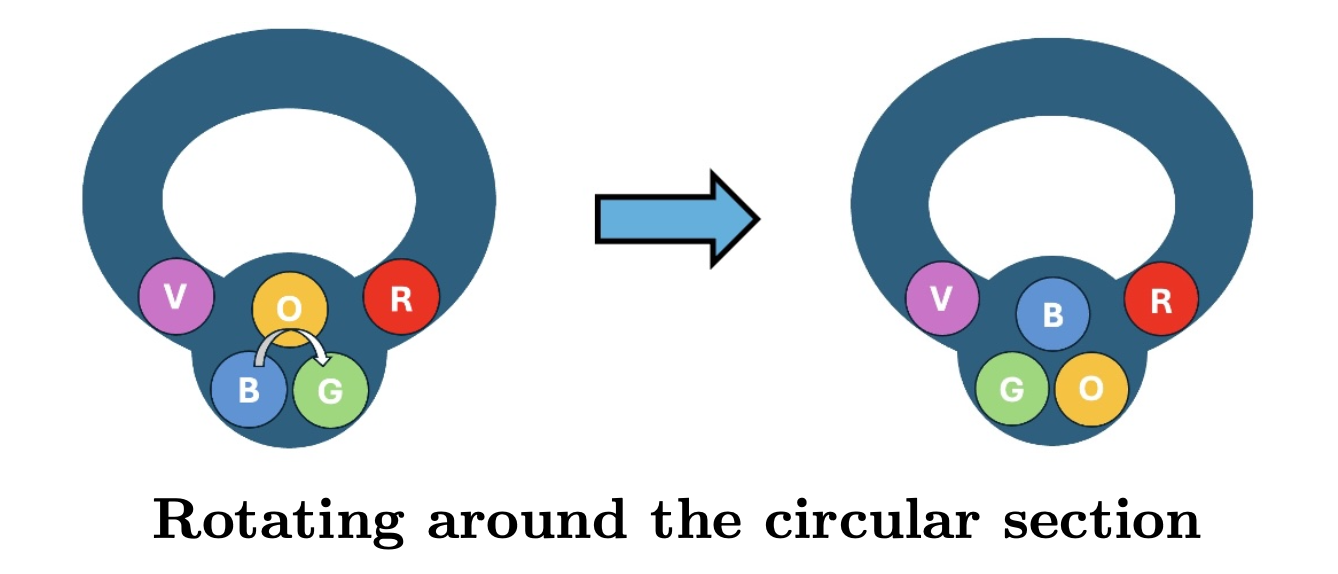
\includegraphics[width=7cm]{circular.png}
        \vspace{-0.3cm}
    \end{figure}
    \begin{figure}[h]
        \centering
        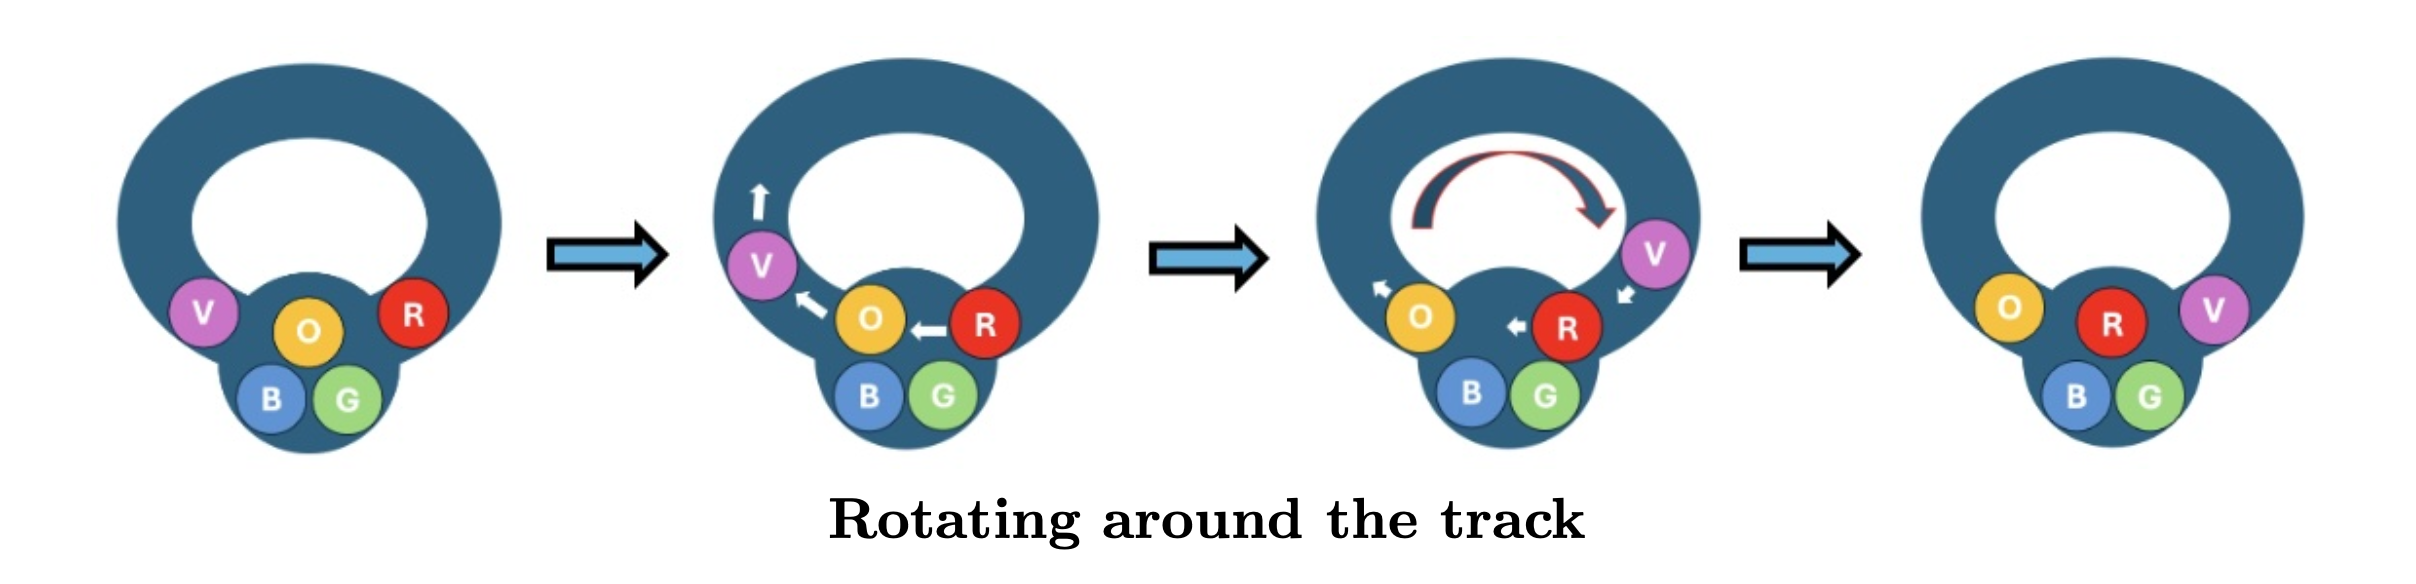
\includegraphics[width=12cm]{track.png}
        \vspace{-0.3cm}
    \end{figure}

    \textbf{(a)} The permutation given is $[3, 2, 1, 5, 4] = (1\ 3)(4\ 5)$ which is even, and can be reached with the moves $CTCCTTCT$:
    \begin{align*}
    &[1, 2, 3, 4, 5] \\
    \text{apply } C \rightarrow &[1, 4, 3, 5, 2] \\
    \text{apply } T \rightarrow &[4, 3, 1, 5, 2] \\
    \text{apply } C \rightarrow &[4, 5, 1, 2, 3] \\
    \text{apply } C \rightarrow &[4, 2, 1, 3, 5] \\
    \text{apply } T \rightarrow &[2, 1, 4, 3, 5] \\
    \text{apply } T \rightarrow &[1, 4, 2, 3, 5] \\
    \text{apply } C \rightarrow &[1, 3, 2, 5, 4] \\
    \text{apply } T \rightarrow &[3, 2, 1, 5, 4]
    \end{align*}

    \textbf{(b)} The permutation given is $[1, 2, 3, 5, 4] = (4\ 5)$ which is odd, so it is impossible to reach it using our operations. \\

    \textit{Extension and remarks:} Since the operations are even, no odd permutations can be reached. It remains to show whether all even permutations are able to be reached with our operations. As even permutations are made from applying pairs of transpositions, this can be done by showing all pairs of transpositions are able to be generated by our operations.

    First, let $(a\ b\ c)$ denote a 3-cycle, meaning that $\sigma_a = b, \sigma_b = c$, and $\sigma_c = a$. We see that operation $C$ corresponds to $(2\ 5\ 4)$ and operation $T$ corresponds to $(1\ 3\ 2)$. For a pair of distinct transpositions, there are 2 cases: they share no elements or one element in common. For the first case, we have $(a\ b)(a\ c) = (a\ b\ c)$ and for the second we have $(a\ b)(c \ d) = (a\ b\ c)(a\ d\ c)$.

    Now, the problem is equivalent to generating all 3-cycles, which can in turn generate all pairs of transpositions and so all even permutations. We provide an extension to the setup of this problem on arbitrarily sized permutations.
    
    Let $S$ be a set of 3-cycles acting on the set of elements $[n] = \{1, 2, \dots, n\}$. Let the \textit{cycle graph} of $S$ be the undirected graph formed where an edge exists between vertices $u$ and $v$ if and only if they both appear in some cycle in $S$. As a generalization, we show that if the cycle graph of $S$ is connected (meaning it is possible to reach every vertex from any starting vertex), then it is possible to generate all 3-cycles using $S$. \\

    \textbf{Lemma:} Let $T$ be a subset of $S$ which acts on the set of elements $X\subset [n]$. Suppose it is possible to generate all even permutations of $X$ using the 3-cycles in $T$. Let $\tau = (u\ v\ w)$ be a 3-cycle with $u\in X$ and at least one of $v, w\notin X$. Then, it is possible to generate all even permutations of $X\cup \{v, w\}$ using the 3-cycles in $T$ and also $\tau$.
    
    \textit{Proof:}  We split into two cases.

    \textbf{Case 1:} $v, w\notin X$.

    First we can generate all 3-cycles of the form $(a\ v\ w)$ and $(a\ w\ v)$ where $a \in X$. Let $(a\ b\ u)$ be a 3-cycle in $T$. Then it can be seen that, $$(a\ u\ b)(u\ v\ w)(a\ b\ u) = (a\ v\ w) \text{ and } (a\ u\ b)(u\ v\ w)(u\ v\ w)(a\ b\ u) = (a\ w\ v).$$
    To calculate the above cycles, one can track the locations of the affected elements, for example like so for the first equality:
    \begin{center}
        \begin{tabular}{|c c c c c |c|} 
            \hline
            $a$ & $b$ & $u$ & $v$ & $w$ & Cycle\\ 
            \hline\hline
            $\sigma_a$ & $\sigma_b$ & $\sigma_u$ & $\sigma_v$ & $\sigma_w$ & - \\ 
            \hline
            $\sigma_b$ & $\sigma_u$ & $\sigma_a$ & $\sigma_v$ & $\sigma_w$ & $(a\ u\ b)$ \\ 
            \hline
            $\sigma_b$ & $\sigma_u$ & $\sigma_w$ & $\sigma_a$ & $\sigma_v$ & $(u\ v\ w)$\\ 
            \hline
            $\sigma_w$ & $\sigma_b$ & $\sigma_u$ & $\sigma_a$ & $\sigma_v$ & $(a\ b\ u)$\\ 
            \hline
        \end{tabular}
    \end{center}
    Next, we can generate all 3-cycles of the form $(a\ b\ v)$ and $(a\ b\ w)$. This is because $$(a\ v\ w)(b\ w\ v) = (a\ b\ w) \text{ and } (a\ w\ v)(b\ v\ w) = (a\ b\ v).$$
    Therefore, we have shown that we can generate all 3-cycles in $X \cup \{v, w\}$.

    \textbf{Case 2:} Exactly one of $v, w\notin X$.

    Without loss of generality, take $v\in X, w\notin X$. We want to generate all 3-cycles of the form $(a, b, w)$. This is possible as $$(a\ b\ v)(u\ v\ w)(a\ v\ u) = (a\ b\ w),$$ so we are done. $\square$ \\
    
    For a single 3-cycle $(a\ b\ c)$, we can easily generate all 3-cycles involving itself: the only other one is $(a\ c\ b) = (a\ b\ c)(a\ b\ c)$. Then, since the cycle graph is connected, we can repeatedly use our above Lemma to generate all possible 3-cycles acting on larger sets of elements, until we generate all 3-cycles acting on $[n]$. This is equivalent to generating all pairs of transpositions, which in turn allows us to generate all even permutations of $[1, 2, \dots, n]$. 
    
    Returning to the problem, clearly the cycle graph of $\{C, T\} = \{(2\ 5\ 4), (1\ 3\ 2)\}$ is connected on $[5]$, so indeed we can generate all even permutations of $[1, 2, 3, 4, 5]$. \\

    Since a similar problem was posed last year, I decided to go into much more depth regarding permutation parity this time. I debated presenting parity using a linear algebra approach as the argument with determinants is very elegant, as well as a cycle counting approach, but I decided on the combinatorial one which to me is the most accessible. Similarly for the extension (which may have been overkill) I had ideas of using some group theory terms like the alternating group $A_n$ and symmetric group $S_n$, but that was quickly shut down as it simply wasn't necessary.
    
    \newpage
    \hyperref[sec:contents]{\section*{Problem 4}}
    \label{sec:p4}
    Instead of displaying a number from $\{1, 2, 3, \dots, p\}$, consider another display that takes the display from the $p$-machine and decreases the number by $1$ (keeping the same color). Thus, it displays a number from the set $\{0, 1, 2,\dots, p\}.$ Now, the rules for turning the crank one full turn on the $p$-machine and reading the new display are:
    \begin{itemize}
        \item[--] if the square is red and the displayed number is less than $p - 1$, then the number is increased by one, and if the square is red and the displayed number is $p - 1$, then the number changes to $0$.
        \item[--] if the square is black and the number is less than $p − k$, then the number increases by $k$, and if the number is greater than or equal to $p − k$, then it decreases by $p − k$.
    \end{itemize}
    We first claim that for this new machine, when the square is red and the displayed number is $a$, then turning the crank once changes the number to $a + 1 \pmod p$.
    
    \textit{Proof:} If $a < p - 1$, then $a + 1 < p$ so the above operation increases the number by $1$ to get a result less than $p$. 
    
    If the displayed number is $p - 1$, then by the above operation, we increase by 1 to get $p \equiv 0 \pmod p$. This is equivalent to the operation given in the problem statement. $\square$ \\

     Next we claim that when the square is black and the displayed number is $a$, then turning the crank once changes the number to $a + k \pmod p$.

     \textit{Proof:} If the displayed number is less than or equal to $p - k$, then the above operation increases the number by $k$ to get a $a + k \pmod p$ not exceeding $p$.
     
     If the displayed number is greater than $p - k$, then let it be $p - k + b$ where $0 < b \leq k$. Then by the above operation, the screen now displays $(p - k + b) + k \equiv p + b \equiv b\pmod p$ which is the original number decreased by $p - k$, so the above operation is equivalent to the operation given in the problem statement. $\square$ \\

     From this, note that when the square is red, then the operation of turning the crank is equivalent to turning the crank when the square is black and $k = 1$.\\

     \textbf{(a)} We claim that a program $k$ is successful if and only if $k < p$. Suppose the display shows $i$ and we want to display $j$.
     
     We first show that this is sufficient. If the square is red, take $k = 1$, otherwise use the given value of $k$, and consider the minimum positive solution for $n$ of $nk\equiv 0 \pmod p$. This value of $n$ is such that turning the crank $n$ times starting from $i$ will return the display to $i$, and as $n$ is minimal, the displayed numbers after $0, 1, \dots, n - 1$ turns will be pairwise distinct. 
     
     Since $p$ is prime and $k < p$, $\gcd(p, k) = 1$, so the above equation is equal to $n\equiv 0 \pmod p$ which has minimal solution $n = p$. As $p$ distinct numbers will be displayed before the $p$-th turn, the numbers $\{0, 1, 2, \dots, p - 1\}$ must all appear. As $j$ is in that set, it is possible to reach $j$.\\

     We now show that $k < p$ is necessary. Suppose $k = p$. Then, if the square is black, then the turning the crank from $i$ changes the number to $i + p \equiv i \pmod p,$ so the number is constant. Therefore, it is impossible to reach a different number in this case. \\

     \textbf{(b)} We claim that a program $k$ is special if and only if $k = 1$ or $k = p - 1$. From the above part, this will also make it successful.

     We first show that this is sufficient. Let the starting number be $a$. If the square starts red, toggling the switch and turning the crank once results in $a + k \pmod p$. Also, turning the crank $k$ times and toggling the switch results in $a + k \pmod p$. This preserves the special property regardless of $k$. 
     
     If the square starts black, toggling the switch and turning the crank once results in $a + 1\pmod p$. Also, turning the crank $k$ times and toggling the switch results in $a + k^2 \pmod p$. For these to be equivalent, we must have
     $$k^2 \equiv 1 \pmod p.$$
     When $k = 1$, this is clearly true, and when $k = p - 1$, $k \equiv -1 \pmod p$, so the above is also true. As $1 < p$ and $p - 1 < p$, for these values of $k$ the program is also successful.\\

     We now show that this is necessary. For $k^2\equiv 1 \pmod p$, $p | k^2 - 1 = (k + 1)(k - 1)$. As $p > 2$, it cannot divide both (as this would mean it would divide their difference of 2), so one of $p | k + 1$ and $p | k - 1$ is true. 
     
     If $p|k + 1$, then as $2\leq k + 1 \leq p + 1$, the only multiple of $p$ in the range is $p$, so it must be that $k = p - 1$.

     If $p | k - 1$, then as $k - 1 < p$ for all possible $k$, it must be that $k - 1 = 0$, which happens when $k = 1$. Hence the only two special programs are $k = 1$ and $k = p - 1$. \\

     \textit{Extension and remarks:} We can now consider the problem when $p$ is composite. For a program to be successful, our argument relied on the fact that $\gcd(p, k) = 1$, meaning the minimum positive solution to $nk\equiv 0 \pmod p$ was $n = p$. This means that turning the crank $p$ times produces $p$ distinct numbers, meaning all of $0, 1, \dots, p - 1$ are reachable. If $\gcd(p, k) > 1$, then we see that $$\frac{p}{\gcd(p, k)} \cdot k \equiv p \cdot \frac{k}{\gcd(p, k)} \equiv 0 \pmod p,$$
     meaning that the minimum positive solution of $n$ to $nk\equiv 0 \pmod 0$ has $n < p$. Therefore, as only $n$ distinct numbers will be produced while turning the crank, there will be numbers that are not reachable. From this, we see that for a program to be successful, $\gcd(p, k) = 1$, which gives $\phi(p)$ values where $\phi$ is Euler's totient function.\\

     Now consider the conditions for $k$ to be special. Let the prime factorization of $p$ be $p_1^{e_1}p_2^{e_2}p_3^{e_3}\cdots p_n^{e_n}$. Similarly to above, we reach the goal of solving $k^2 \equiv 1 \pmod p$. As $p | (k^2 - 1)$, for each prime factor we have $p_i^{e_i} | (k^2 - 1)$, meaning that $k$ must satisfy
     \begin{align*}
     k^2\equiv &1 \pmod{p_1^{e_1}} \\
     k^2\equiv &1 \pmod{p_2^{e_2}} \\
     &\vdots \\
     k^2\equiv &1 \pmod{p_n^{e_n}}
     \end{align*}
     From this we see that $p_i^{e_i} | (k + 1)(k - 1)$. If $p_i > 2$, then $p_i$ cannot divide both factors as it would divide their difference (as mentioned above), so $k \equiv \pm1 \pmod{p_i^{e_i}}$. If $p_i = 2$ there are more cases. Clearly, if $e_i = 1$, there is only one solution, namely $k \equiv 1\pmod 2$. If $e_i = 2$, then there are two solutions: $k \equiv \pm 1 \pmod{2^2}$. 
     
     Now for $e_i \geq 3$, as $k + 1$ and $k - 1$ have the same parity, we see that they must be both even, which also tells us $\gcd(k + 1, k - 1) = \gcd(2, k - 1) = 2$ by the Euclidean algorithm. So, it is sufficient that $$2^{e_i - 1} | (k + 1) \text{ or } 2^{e_i - 1} | (k - 1),$$ as the other factor will contribute exactly 1 factor of 2. Hence for this case there will be four solutions: $k \equiv \pm 1, 2^{e_i - 1}\pm 1 \pmod{2^{e_i}}$.

     To finish, we have $n$ congruences for $k$ in the form $k \equiv a_i \pmod{p_i^{e_i}}$. For all combinations of choices for $a_i$, there is a unique solution modulo $p$ by the Chinese Remainder Theorem. For example, the special case where $p$ is odd there will be $2^n$ values of special $k$. Finally, as there exists integer $m$ such that $$k^2 - pm = 1,$$ by Bézout's lemma $\gcd(p, k) = 1$, so all special $k$ are also successful.\\
     
     For me, not too complicated of a number theory problem once you play with the operations and realize they are just addition modulo $p$. The generalization adds a little more spice and would be more difficult without prerequisite knowledge.
    
    \newpage
    \hyperref[sec:contents]{\section*{Problem 5}}
    \label{sec:p5}
    Let the cell in the $x$-th column from the left and $y$-th row from the bottom have coordinates $(x - 1, y - 1)$, so the ant starts in the cell $(0, 0)$. For each cell $(x, y),$ assign a weight of $\dfrac{1}{2^{x + y}}$. 
    \begin{figure}[h]
        \centering
        \vspace{-0.3cm}
        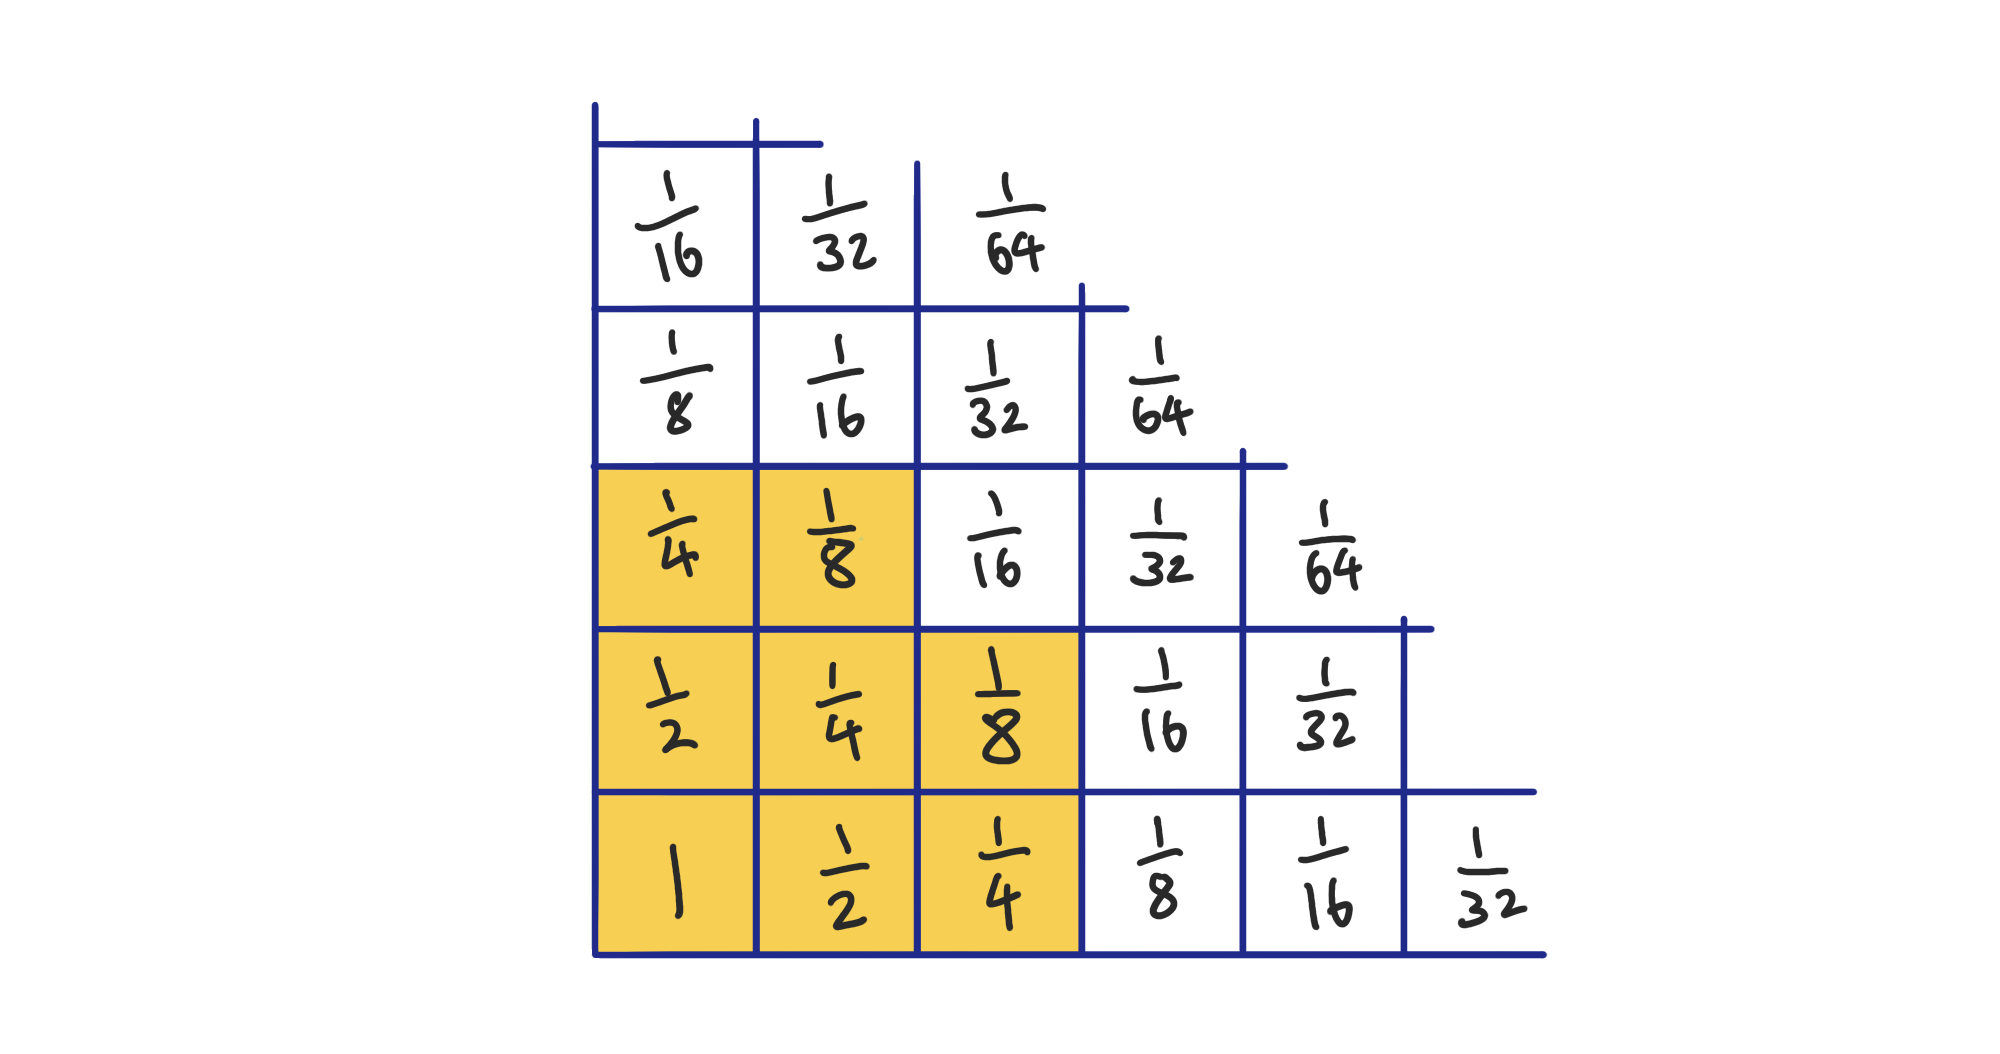
\includegraphics[width=12cm, trim = 0 0.5cm 0 1cm, clip]{antgrid.png}
        \vspace{-0.3cm}
    \end{figure}
    
    Initially the sum of the weights of occupied cells is $1$. When an ant at $(x, y)$ duplicates itself, then the change in the sum of the weights of occupied cells will be $$\left(\frac{1}{2^{(x + 1) + y}} + \frac{1}{2^{x + (y + 1)}}\right) -\frac{1}{2^{x + y}} = \frac{1}{2^{x + y}} - \frac{1}{2^{x + y}} = 0.$$

    Therefore, at all times, the sum of the weights of occupied cells will remain constant as $1$. We can work out the total weight of all cells in the grid by summing infinite geometric series:
    $$\left(1 + \frac{1}{2} + \frac{1}{4} + \cdots\right) + \left(\frac{1}{2} + \frac{1}{4} + \frac{1}{8} + \cdots \right) + \left(\frac{1}{4} + \frac{1}{8} + \frac{1}{16} + \cdots \right) + \cdots$$
    $$= 2 + 1 + \frac{1}{2} + \frac{1}{4} + \cdots = 4.$$
    Furthermore, the sum of the weights of the yellow region is $$1 + \frac{1}{2} + \frac{1}{2} + \frac{1}{4} + \frac{1}{4} + \frac{1}{4} + \frac{1}{8} + \frac{1}{8} = 3.$$
    This tells us the sum of the weights of cells outside the yellow region is $1$. From this, we see that if the ants vacate the yellow region, they must fill \textit{every} cell outside the yellow region to satisfy the sum of the weights of occupied cells being $1$. This is an infinite number of cells, and so for finite $t$ it is impossible that the ants completely vacate the yellow region. \\
    
    \newpage
    \hyperref[sec:contents]{\section*{Problem 6}}
    \label{sec:p6}
    \textbf{(a)} Here is an $A+$ topper with 35 cards, with the layout expanded for clarity:
    \begin{figure}[h]
        \centering
        \vspace{-0.3cm}
        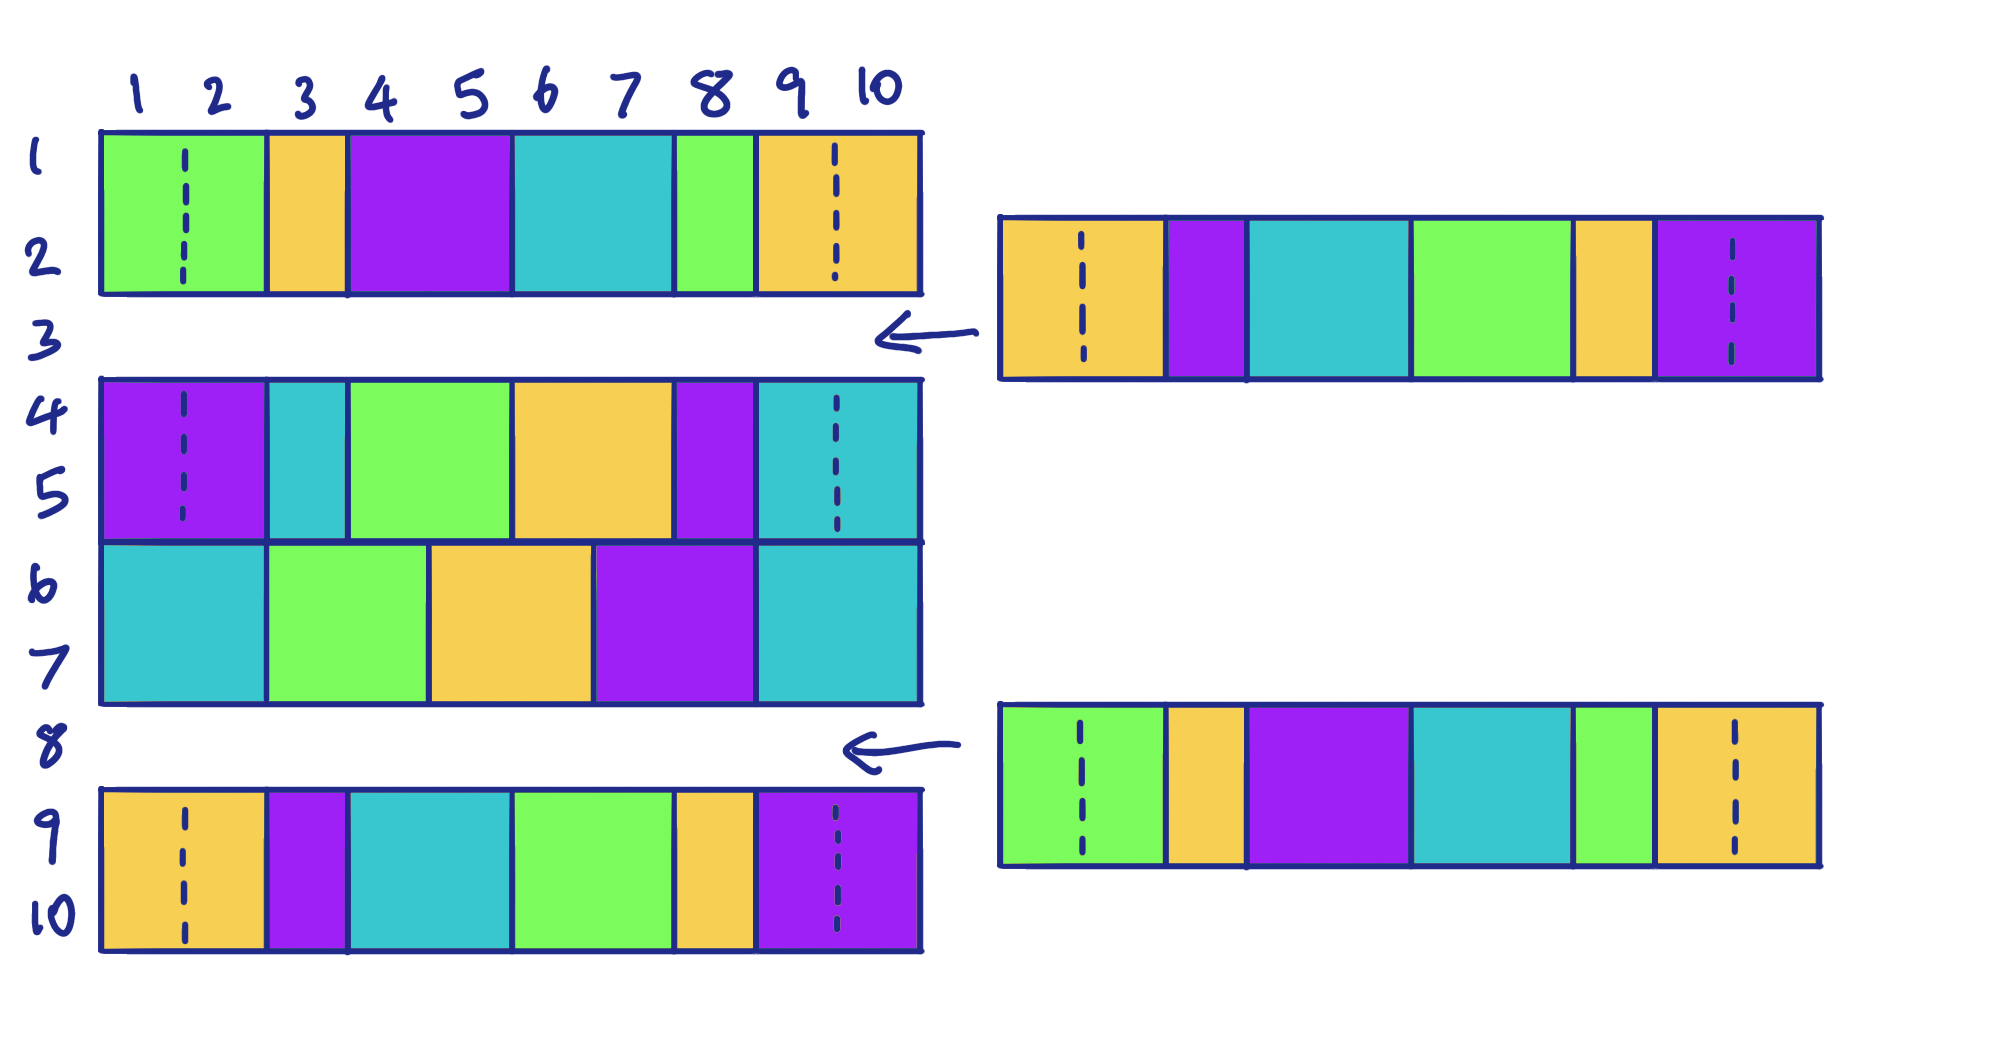
\includegraphics[width=12cm, trim = 0 0.5cm 0 0.5cm, clip]{35topper.png}
        \vspace{-0.5cm}
    \end{figure}
    
    \textbf{(b)} Consider the puzzle on a $2\times10$ grid. We show that an $A+$ topper has at most 6 cards. This is clearly possible as seen in the last row of the above diagram.
    
    Assume for the sake of contradiction that there exists an $A+$ topper with $k > 6$ cards. Then, since each card takes up $2$ columns and cards clearly cannot fully overlap, there will be $2k - 10 \geq 4$ columns that are covered by more than one card. This means the number of columns covered by just one card is at most $6$. However, we must have at least $k \geq 7$ columns that are covered by just one card to satisfy the $A+$ property, which is a contradiction, and so 7 cards is impossible.
    
    Therefore, each two adjacent rows can hold a maximum of 6 cards. There are $9$ such sections on the grid, meaning that an upper bound for the largest $A+$ topper is $6\times 9 = 54$ cards. Hence, every topper with 55 cards is silly.\\
    
    \textbf{(c)} We claim that the largest $A+$ topper has $38$ cards. First, below is a topper with $38$ cards, showing that this number is achievable. 
    \begin{figure}[h]
        \centering
        \vspace{-0.3cm}
        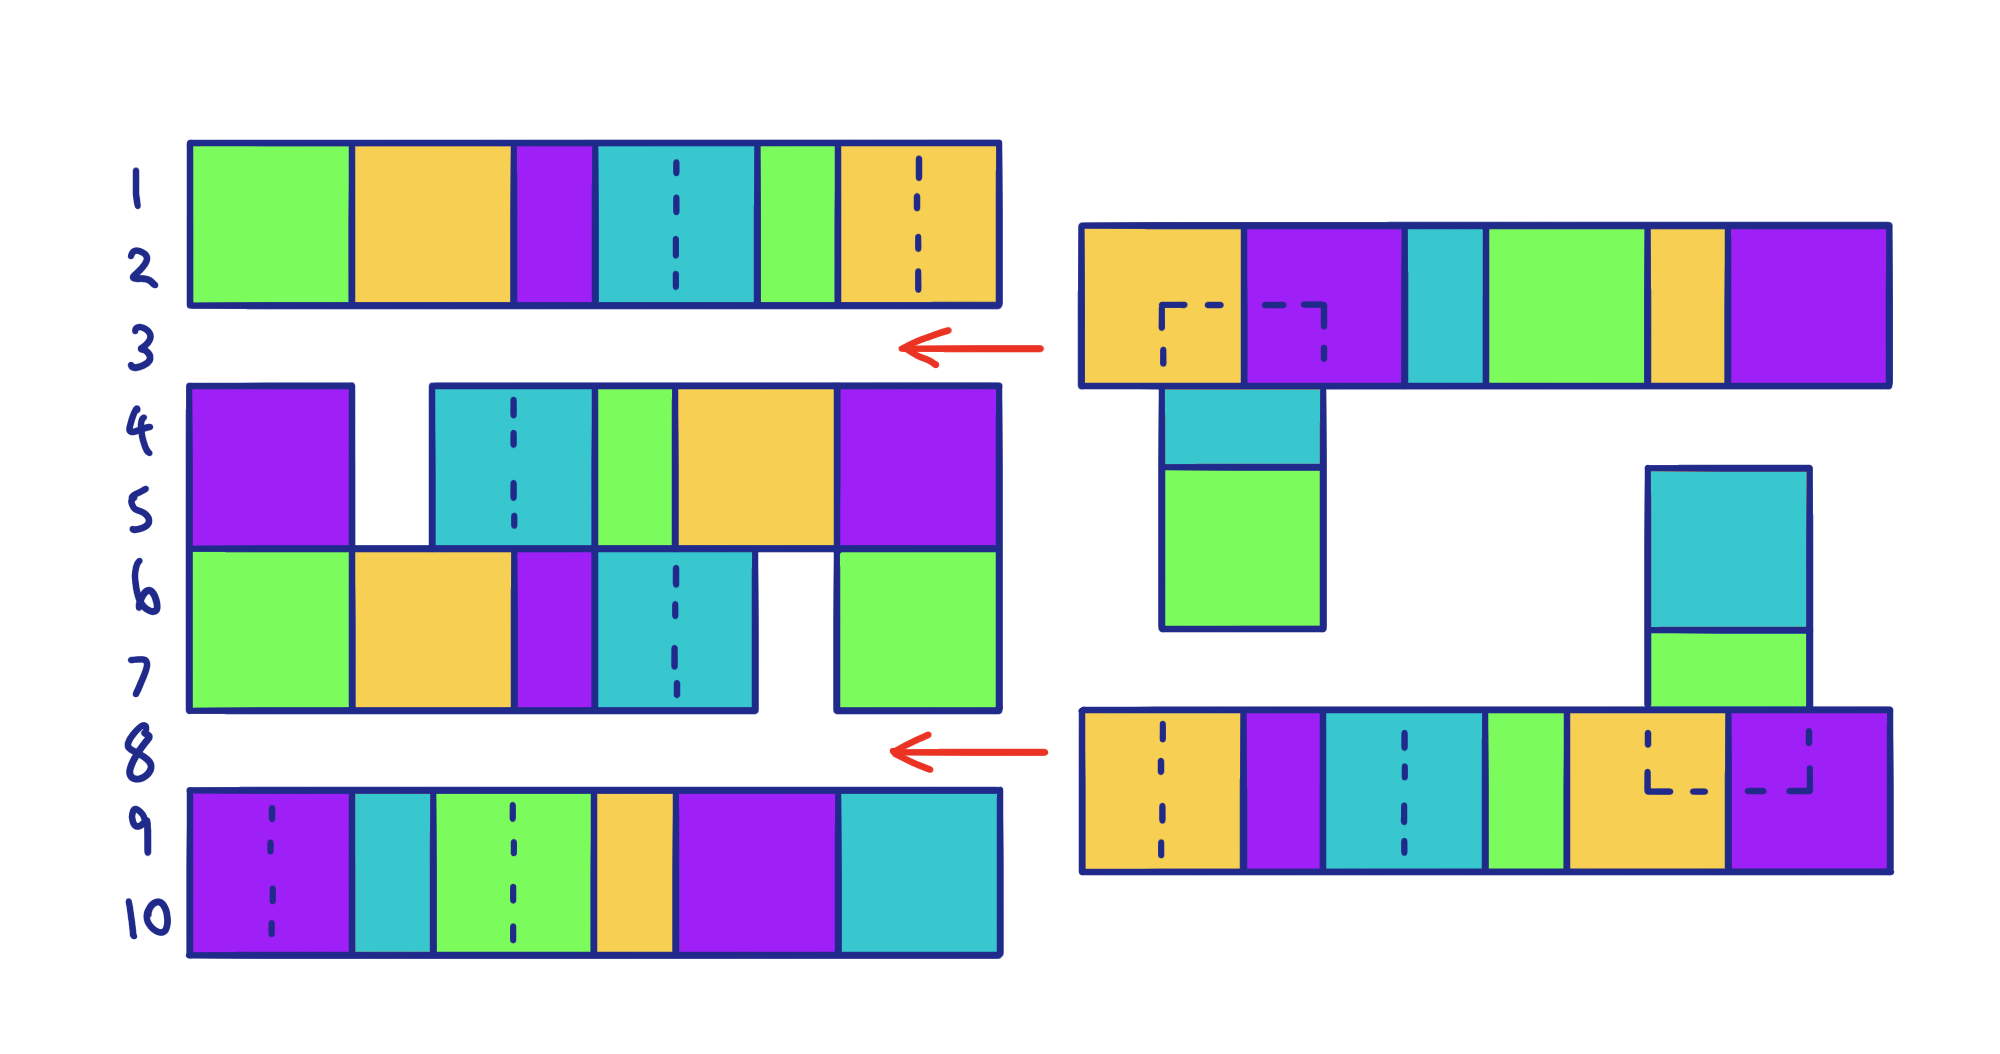
\includegraphics[width=12cm, trim = 0 0.8cm 0 1.3cm, clip]{finalsplit.png}
        \vspace{-0.3cm}
    \end{figure}

    First, we show that the largest $A+$ topper of a $3\times 10$ grid contains $12$ cards. A card can only be placed on rows 1–2 or rows 2–3. Clearly, the top and bottom rows must be covered, and the maximum number of cards we can place in a $2\times 10$ space is 6, so we simply place the maximum number of cards on rows 1–2 and rows 2–3, achieving the result.
    
    Similarly, the largest $A+$ topper of a $4\times 10$ grid also contains $12$ cards. Again, we fill rows 1–2 and rows 3–4 with 6 cards as they have to be filled for all configurations regardless. Then, since rows 2–3 are now also fully covered, we cannot place any card onto those two rows as that would violate the $A+$ condition. 
    \begin{figure}[h]
        \centering
        \vspace{-0.3cm}
        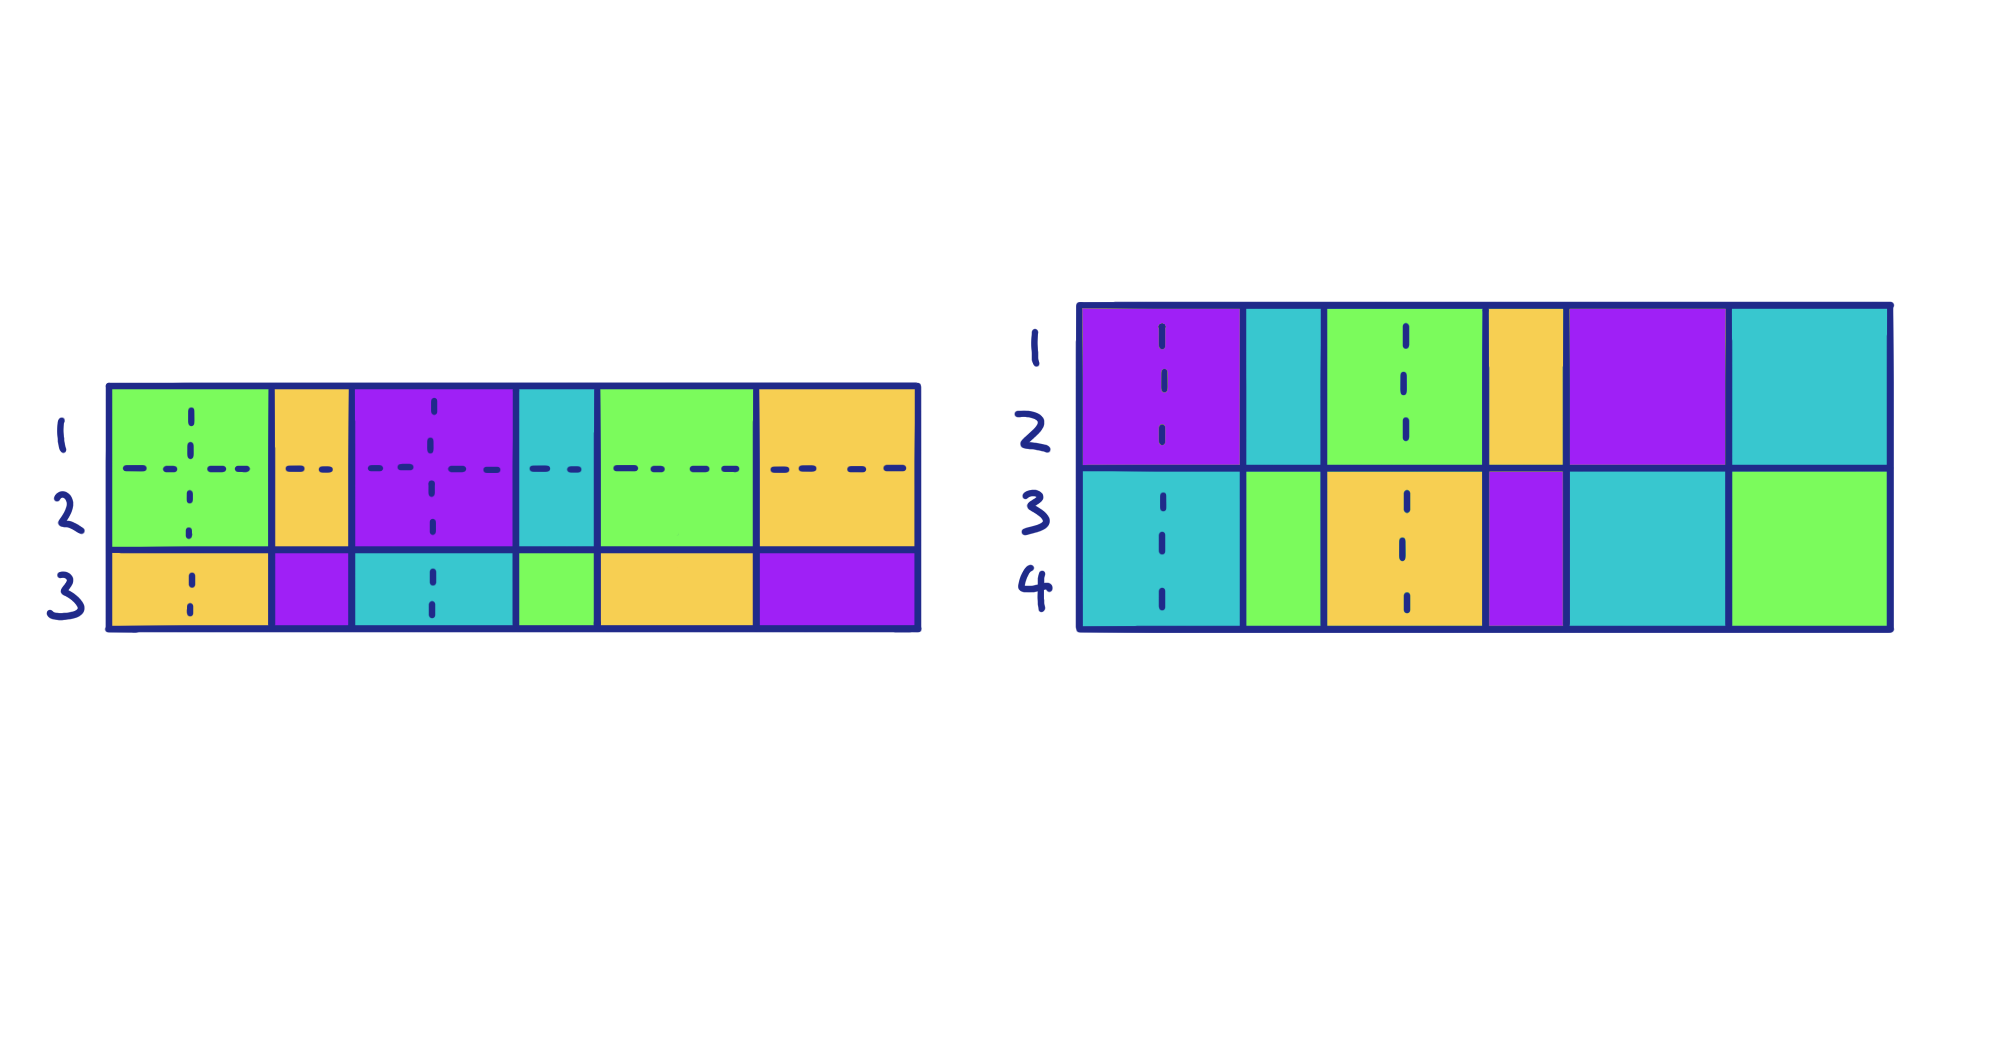
\includegraphics[width=11cm, trim = 0 4cm 0 2.5cm, clip]{threefour.png}
        \vspace{-0.3cm}
    \end{figure}

    Now, we claim that the largest $A+$ topper of a $7\times 10$ grid contains $25$ cards. Consider the $A+$ topper formed by placing the maximal $A+$ topper of a $4\times 10$ grid in rows 1–4 and the maximal $A+$ topper of a $3\times 10$ grid in rows 5–7, as seen below. This has $24$ cards. 
    \begin{figure}[h]
        \centering
        \vspace{-0.3cm}
        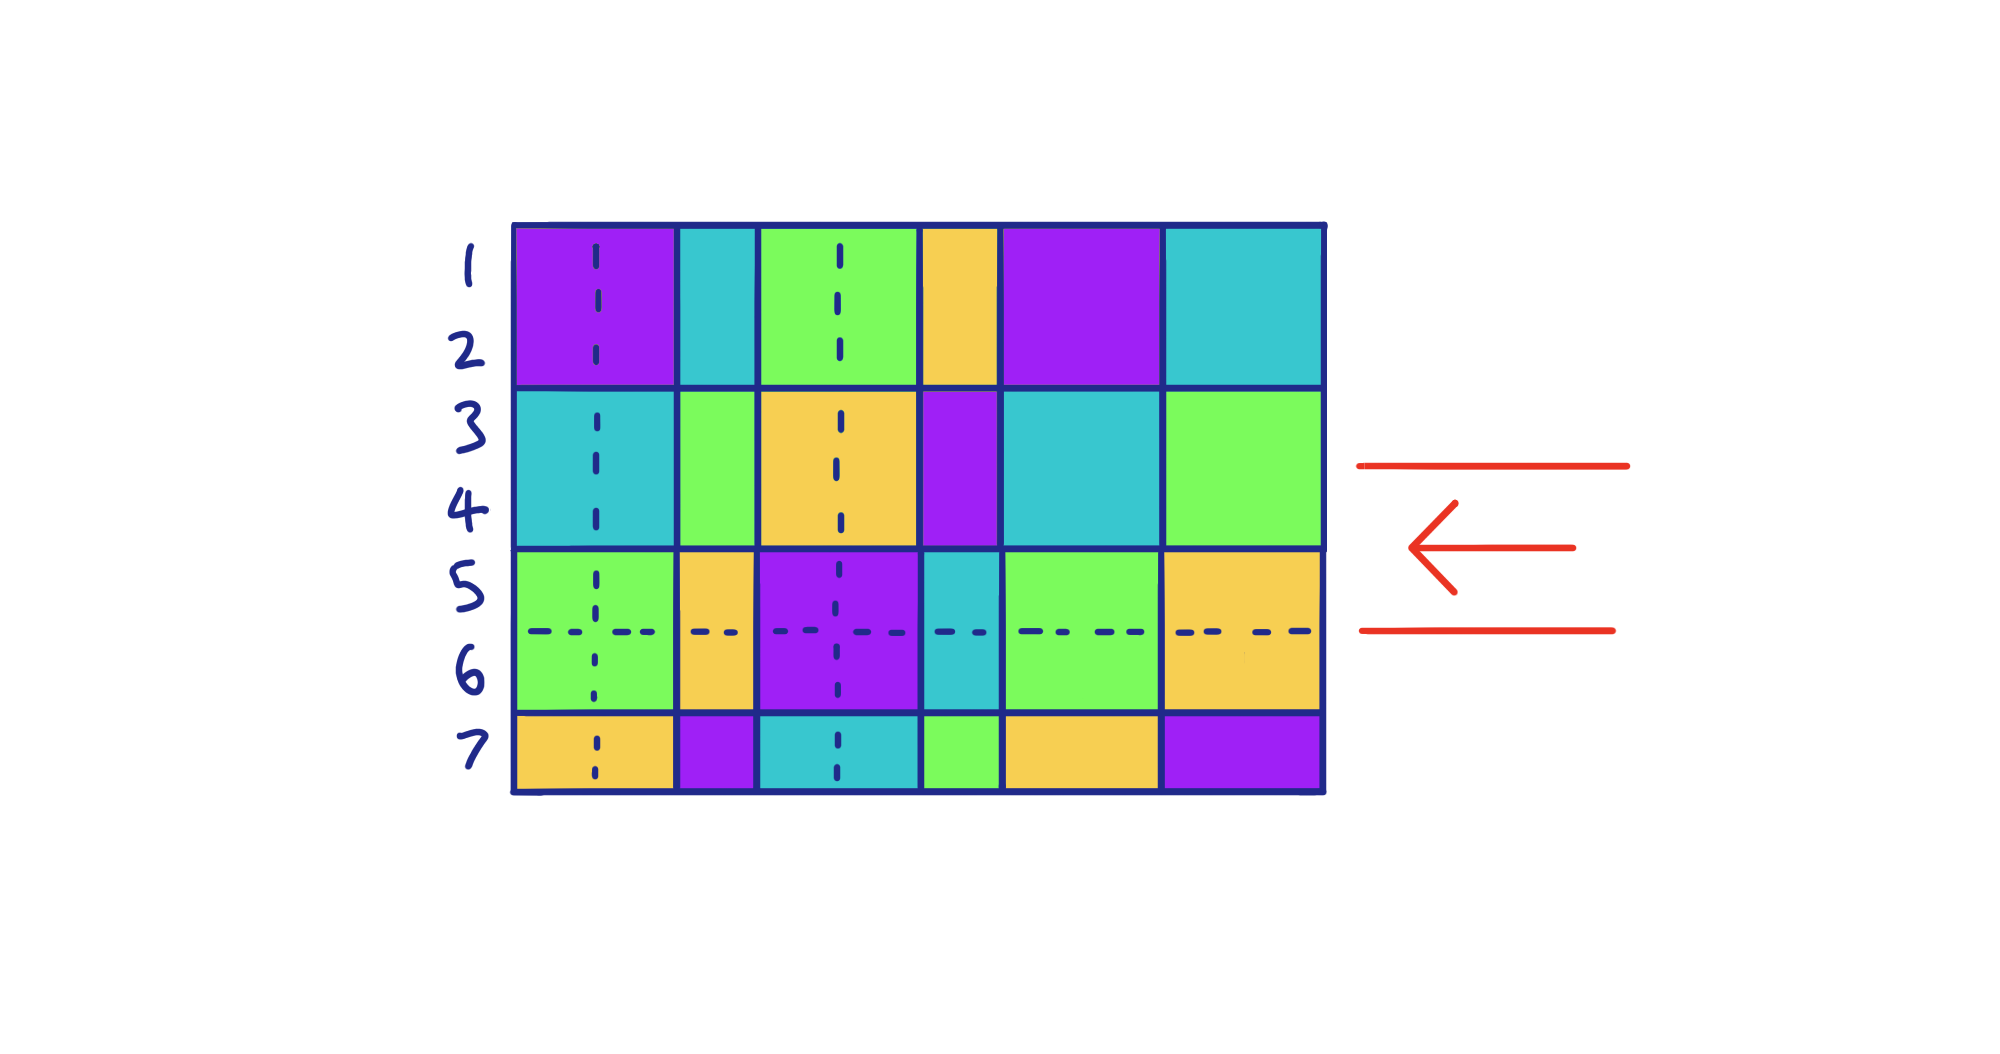
\includegraphics[width=11cm, trim = 0 2.2cm 0 1.8cm, clip]{seven.png}
        \vspace{-0.3cm}
    \end{figure}
    
    If an $A+$ topper has more than $24$ cards, then there must be cards that cover rows 4-5, as otherwise, since no cards span the two regions we simply consider their upper bounds separately to show that we cannot exceed $24$ cards. 
    
    Let us consider the cards placed in rows 4–5. Define the \textit{private cell} of a card to be a cell that is only covered by 1 card. Each card must have at least one private cell, otherwise the configuration is no longer $A+$. Since row 6 is fully covered by the bottommost cards, the cards in rows 5–6 must have their private cells in row 5. Assume that cards in rows 4–5 have their private cell in row 4, so there is more freedom to place cards in rows 5–6. 
    
    We claim that at most 7 cards can be placed in rows 4–6 for the rest of the grid to be able to be filled. Assume the contrary, that it is possible to place 8 cards in those rows. Notice that each column can contain at most one private cell. Consider consecutive ``runs" of columns that contain private cells. The maximum length of a run is 4 columns, shown below in the top left. If we have two of these runs together, then the resulting configuration is 11 cells wide. Therefore, for 8 cards to be possible, there must be exactly three runs, and the two extra columns must separate runs and not be on the boundaries. It is only possible to create runs of length 1 and 2 that do not take more columns on one side, shown below in the bottom left. Therefore, we must have runs of length 2, 4, and then 2. However, this creates the following configuration in the top right, and we see that the red cells cannot be filled, so 7 cards is indeed the maximum (example in the bottom right).
    \begin{figure}[h]
        \centering
        \vspace{-0.3cm}
        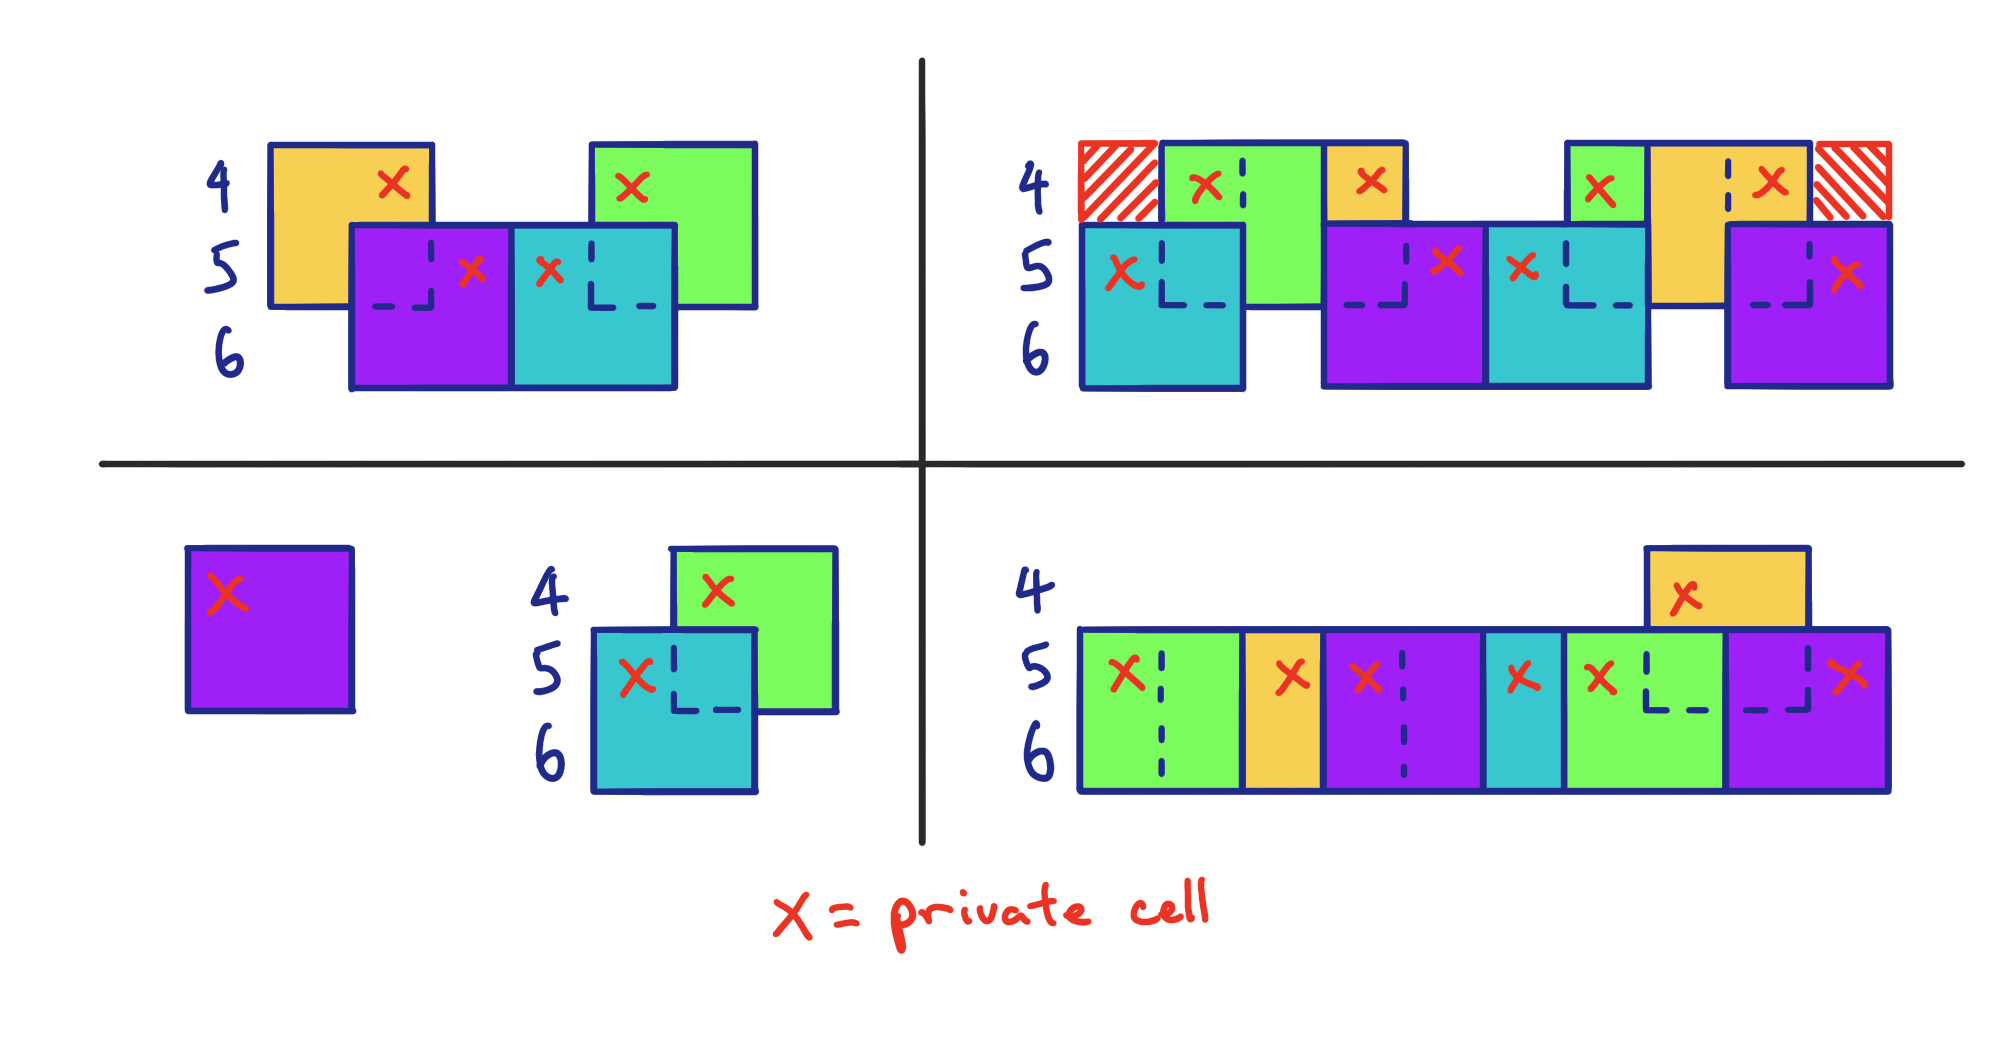
\includegraphics[width=11cm, trim = 0 1cm 0 1cm, clip]{privateruns.png}
        \vspace{-0.3cm}
    \end{figure}
    
    As the cards in rows 4–5 will have private cells in row 4, to maximize the number of cards we can potentially place in rows 1–4, we only place one cell in rows 4–5. However, since we must have a private cell in row 4, we cannot have 6 cards in rows 3–4. This is because with 6 cards, we can only leave columns 1, 4, 7, and 10 empty, while the private cell that extends into row 4 cannot be in those positions (see below).
    \begin{figure}[h]
        \centering
        \vspace{-0.3cm}
        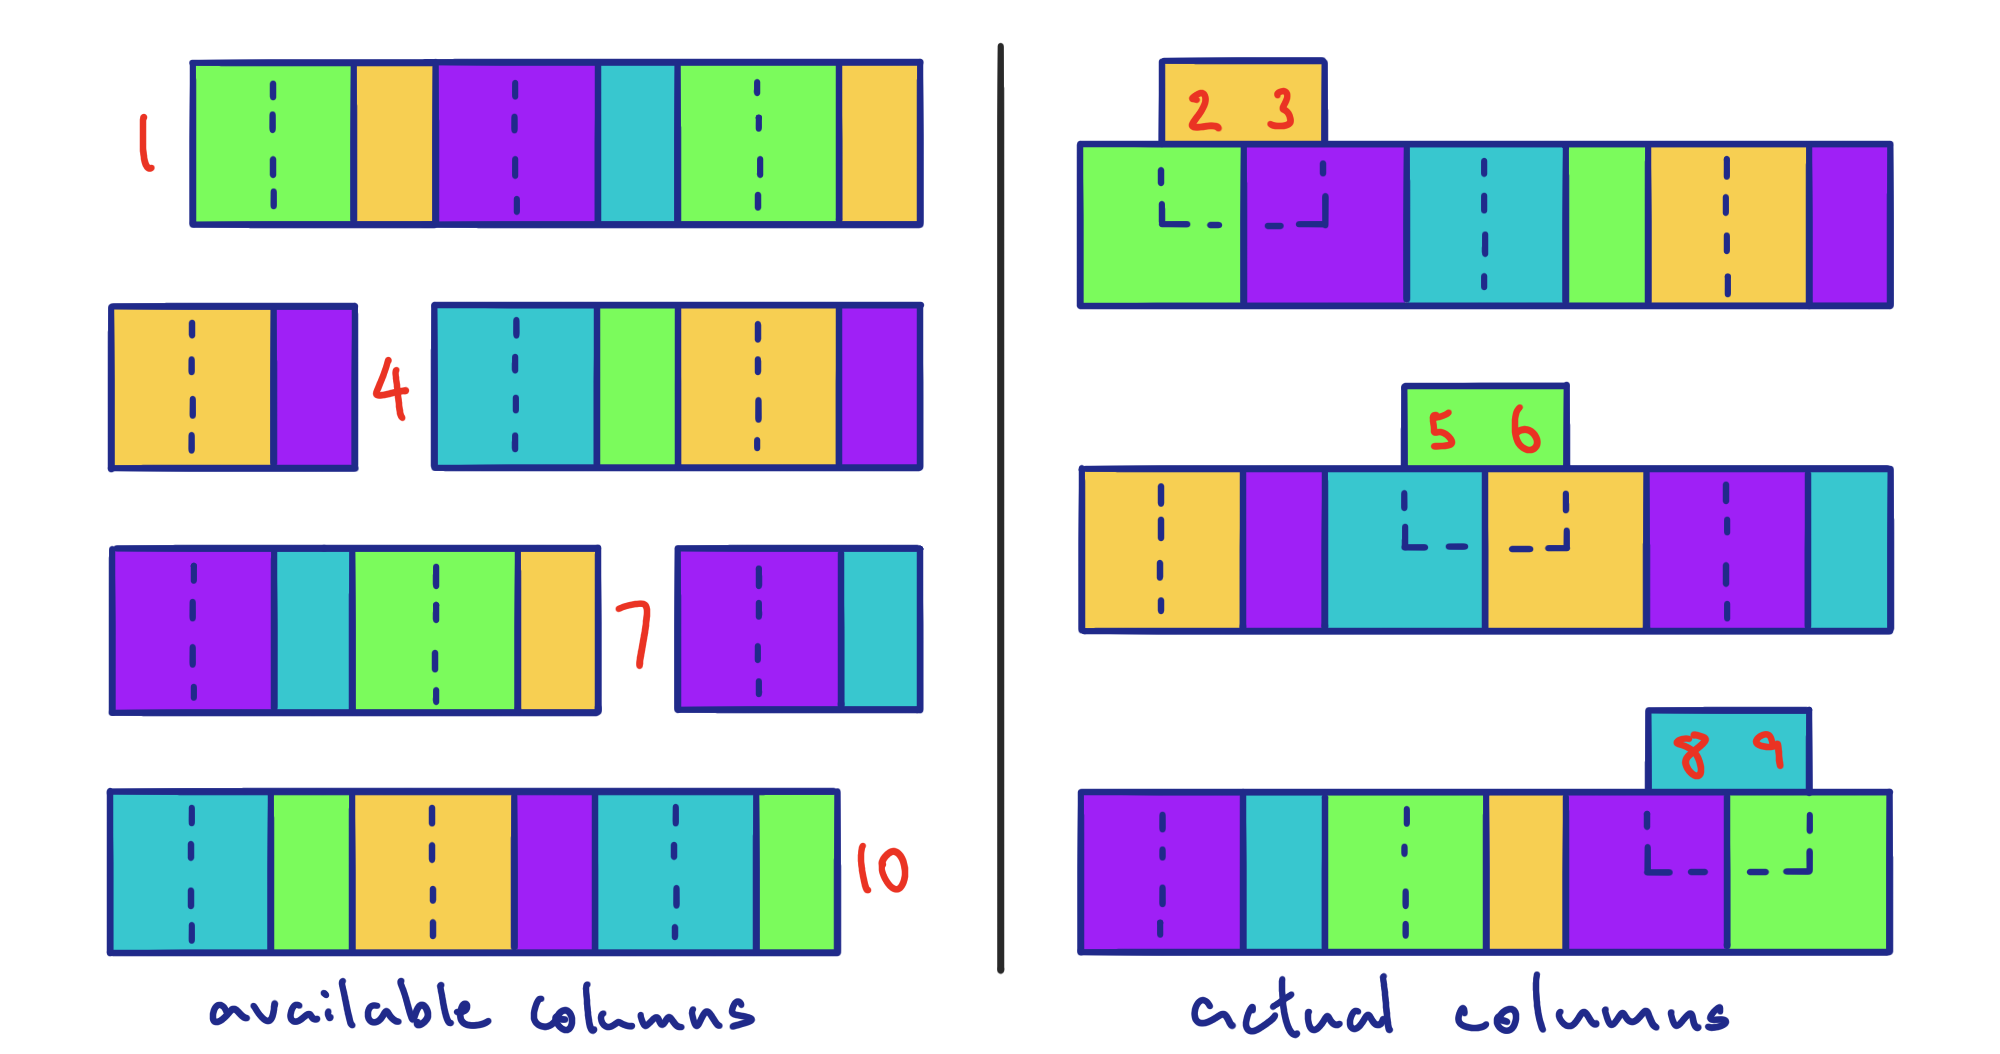
\includegraphics[width=11cm, trim = 0 0cm 0 0.5cm, clip]{incompatible.png}
        \vspace{-0.3cm}
    \end{figure}
    
    Therefore, we can only place 5 cards in rows 3–4. We can create an empty column as shown below and to the right. This will allow us to place a card in rows 2–3 so that there are 12 cards in rows 1–4. As rows 1–2 must be fully covered and rows 3–4 must contain no more than 5 cards, we can only insert one card in rows 2–3, so this is indeed the maximum.
    \begin{figure}[h]
        \centering
        \vspace{-0.3cm}
        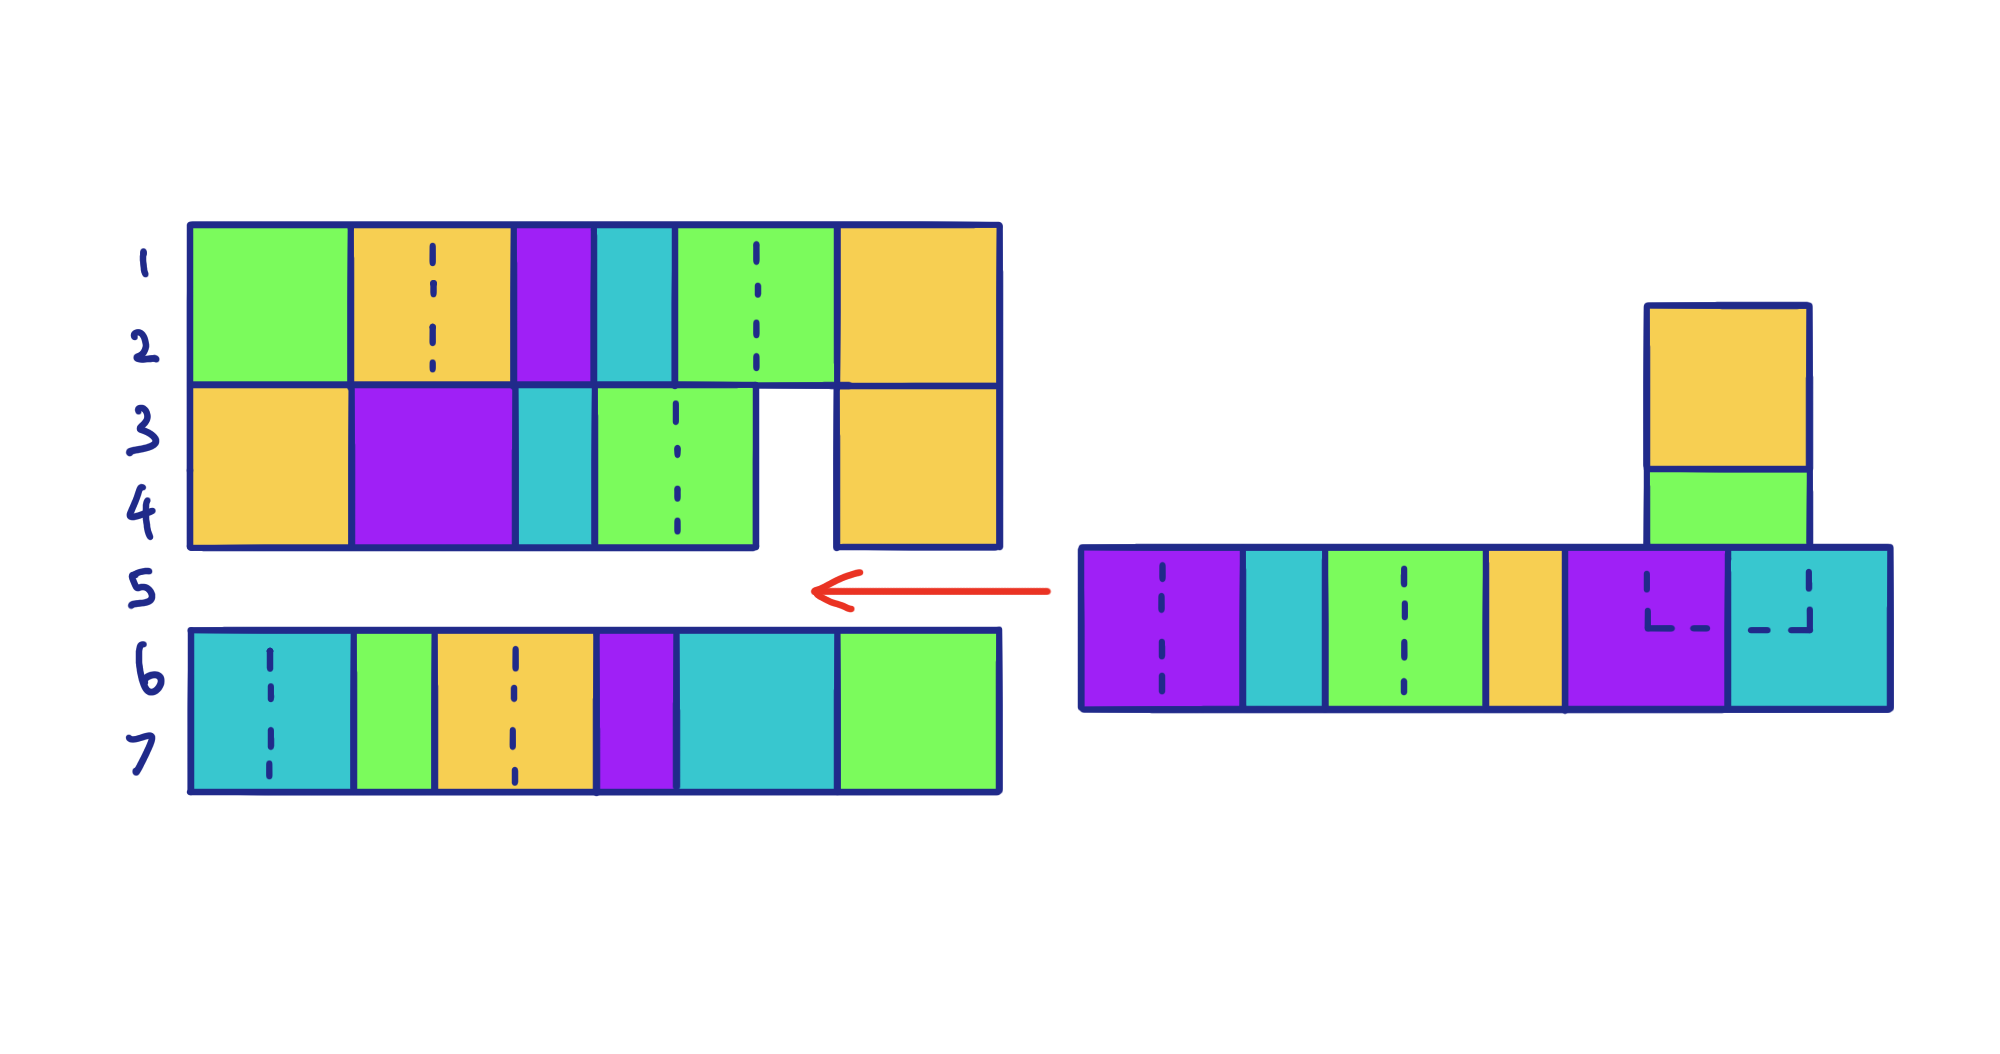
\includegraphics[width=11cm, trim = 0 2.5cm 0 1.8cm, clip]{better.png}
        \vspace{-0.3cm}
    \end{figure}

    Now, we can use similar logic for a $10\times 10$ grid, by placing the maximum $A+$ topper of a $3\times 10$ grid in the first three rows and then placing our new $A+$ topper for the $7\times 10$ grid in the bottom rows, and then finding that we can once again place an extra card than the separate bounds allow. Therefore, the maximal $A+$ topper for a $10\times 10$ grid contains $38$ cards. Here is the expanded view:
    \begin{figure}[H]
        \centering
        \vspace{-0.3cm}
        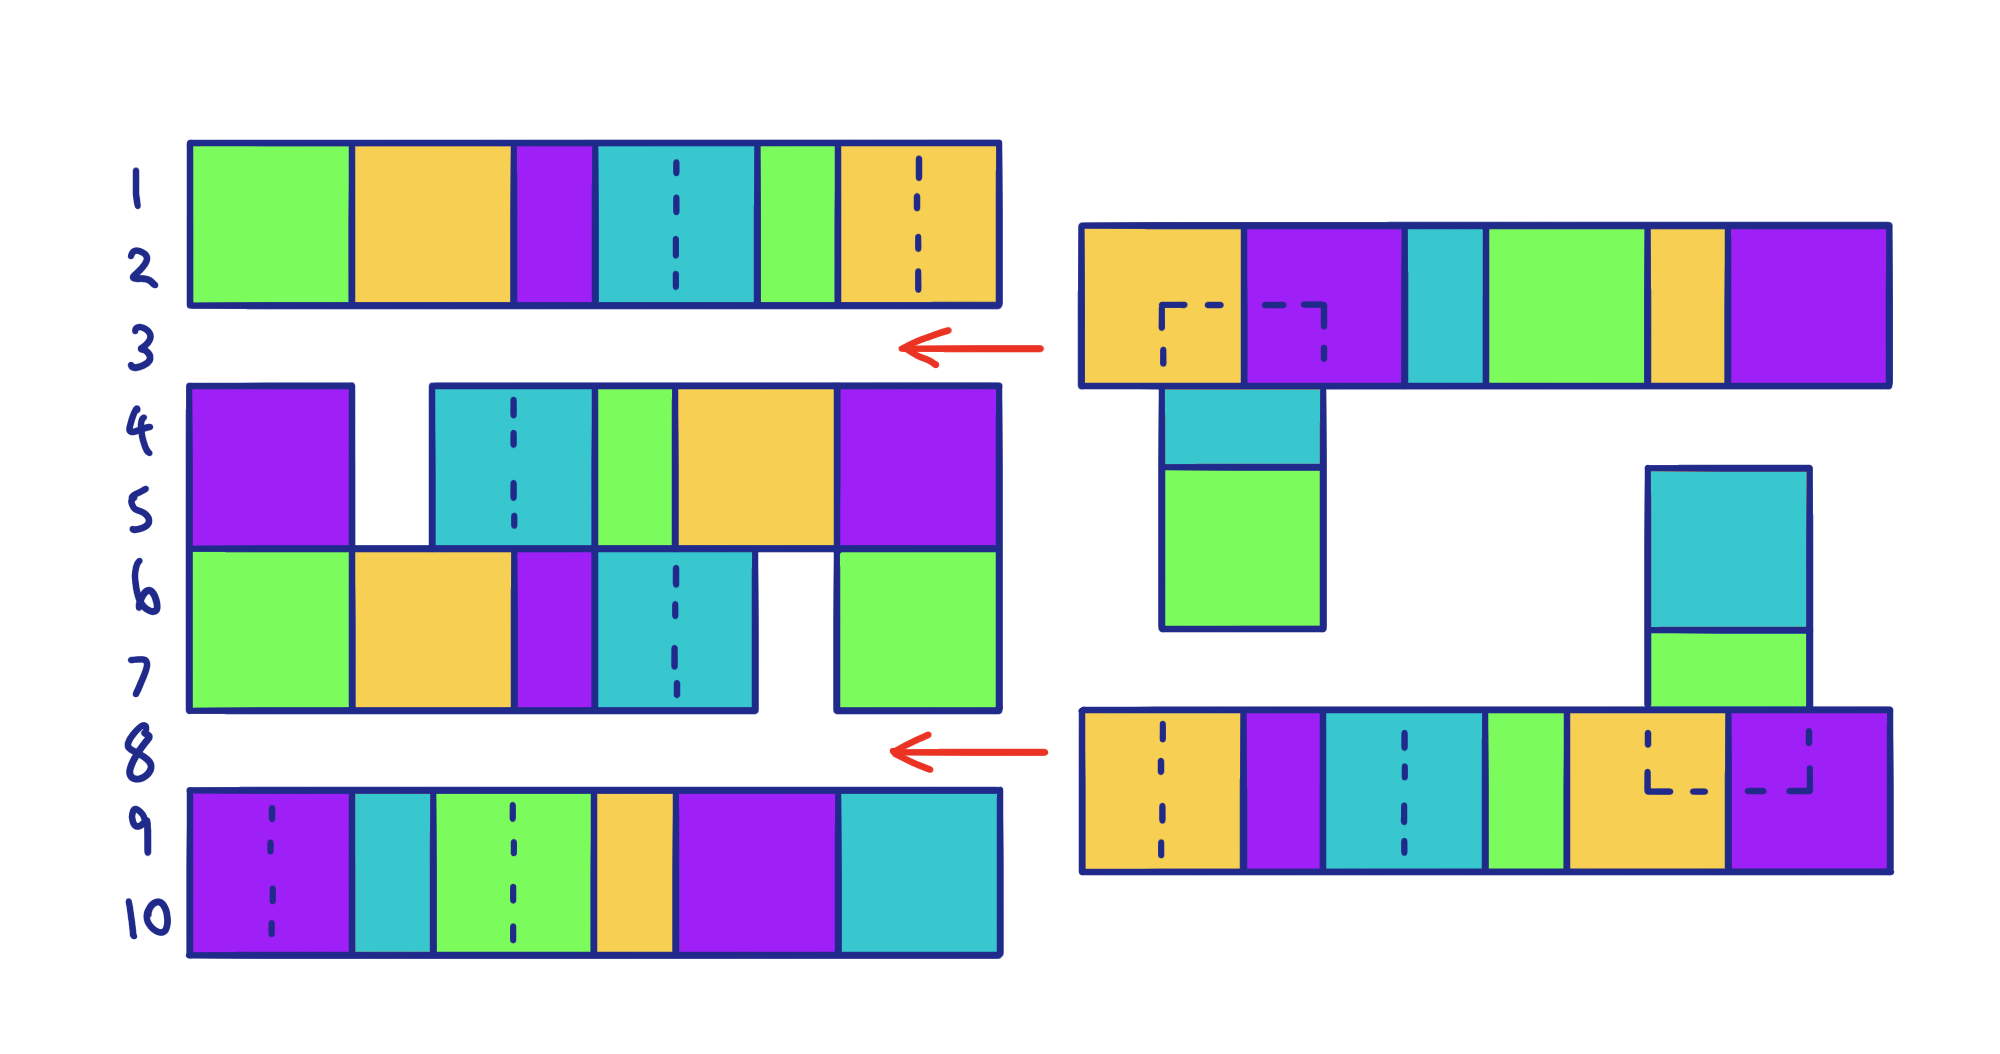
\includegraphics[width=11cm, trim = 0 0.8cm 0 1.3cm, clip]{finalsplit.png}
        \vspace{-0.3cm}
    \end{figure}

    Here is the combined view, with private cells marked:
    \begin{figure}[H]
        \centering
        \vspace{-0.3cm}
        
\includegraphics[width=12cm, trim = 0 1cm 0 0.5cm, clip]{final.png}
        \vspace{-0.3cm}
    \end{figure}
    
    \textit{Extension and remarks:} In general, for a $2\times n$ grid, as we cannot have three cards placed consecutively partially overlapping each other, we find that (for example by induction) the maximum number of cards we can place is $f(n) = \left\lfloor{\frac{2n}{3}}\right\rfloor$. Therefore, for an $n\times m$ grid, then the maximal $A+$ topper has a lower bound of at least $f(n)f(m)$ cards, which can be placed in a fashion similar to the Cartesian product of a $2\times n$ topper and a $2\times m$ topper. Below is an example for $n = 11, m = 14$:

    For the upper bound, first consider the case when $n$ and $m$ are both multiples of $3$. It can be shown by induction that our lower bound is also the upper bound, as by a similar reasoning to the above, placing any cards across the boundary of two sections will result in the removal of two cards above and below the boundary. Then, we can consider all different cases for $n$ and $m \pmod 3$. Without loss of generality take $n > m \pmod 3$. As with the $10\times 10$ grid, we can place all ``isolated" rows in the center, then add overlapping rows on either side to try and add extra cards and show the upper bound. This requires delicate casework but I believe that the upper bound is indeed like the one found in part c), that is, $f(n)f(m) + 2$. \\

    I quickly solved the first two parts, but then became convinced that $36$ was the largest $A+$ topper. I subsequently tried for over two weeks to show this, to no avail, as the casework for the positioning simply became too complicated. Finally, I began to doubt my initial answer and looked for alternatives. Mere days before the deadline, I finally realized the optimal strategy and finished the problem off. I still believe there is a better solution than what I have done, and the generalization does feel sketchy, but I am quite confident that what I have done within the scope of the problem is correct.
    
\end{document}